% TWC journal layout; the official class is kept separate to preserve earlier drafts.
% Template provenance is recorded in journal_template/README.md.
\documentclass[10pt,journal,letterpaper]{journal_template/IEEEtran}
\usepackage{cite}
\usepackage{amsmath,amssymb,amsfonts}
\usepackage{array}
\usepackage{amsthm}
\usepackage{bm}
\usepackage{enumitem}
\usepackage{algorithmic}
\usepackage{graphicx}
\usepackage{textcomp}
\usepackage{xcolor}
\usepackage{mathtools}
\usepackage{threeparttable}
\usepackage[caption=false]{subfig}
\usepackage{float}
\usepackage{overpic}
\usepackage{pifont}
\usepackage{color}
\usepackage{algorithm}
\usepackage{hyperref}
\usepackage{cleveref}
\usepackage{booktabs}
\usepackage{multirow}
\usepackage{makecell}
\usepackage[normalem]{ulem}
% Revision markup: confirmed edits are blue; current additions are red;
% current deletions are red with strikethrough.
% Deletion baseline: submitted main.tex, not intermediate revision drafts.
% After approval, replace the current comment's \currentrev wrappers with \rev.
\colorlet{revisioncolor}{blue}
\colorlet{deletioncolor}{red}
\newcommand{\rev}[1]{\textcolor{revisioncolor}{{}#1}}
\newenvironment{revblock}{\color{revisioncolor}}{}
% The empty group preserves any explicit leading space inside the marker.
\newcommand{\currentrev}[1]{\textcolor{red}{{}#1}}
\newif\ifshowdeletions
%\showdeletionstrue % Use \showdeletionstrue to show the deleted text.
\showdeletionsfalse % Use \showdeletionsfalse to hide the deleted text.
\newcommand{\currentdel}[1]{\ifshowdeletions\textcolor{deletioncolor}{\sout{#1}}\fi}
%TC:macro \currentdel [ignore]
\newcommand{\refalg}[1]{Alg.~\ref{#1}}
\newcommand{\reffig}[1]{Fig.~\ref{#1}}
\newtheorem{theorem}{Theorem}
\newtheorem{proposition}{Proposition}
\newtheorem{lemma}{Lemma}
\theoremstyle{remark}
\newtheorem*{remark}{Remark}

% Use the unmodified journal text area; do not override margins with geometry.

\def\BibTeX{{\rm B\kern-.05em{\sc i\kern-.025em b}\kern-.08em
    T\kern-.1667em\lower.7ex\hbox{E}\kern-.125emX}}
\begin{document}

\title{MEET-COBRA: Machine-learning-based Energy-Efficient proacTive Coordination of handOver, Beamforming and Resource Allocation}

% MeetCobra: ML-based Energy-Efficient inTelligent Coordination of handOver, Beamforming and Resource Allocation
% EAT-COBRA: Energy-efficient AI-based Proactive Coordination of handOver, Beamforming and Resource Allocation
% MEET-COBRA: ML-based Energy-Efficient proacTive Coordination of handOver, Beamforming and Resource Allocation
% MEPOBA/MEPHOBA: ML-based Energy-Efficient Proactive HandOver, Beamforming and Resource Allocation

% \IEEEauthorrefmark{1}
\author{Bowen~Xie, Sheng~Zhou, and Zhisheng~Niu%
\thanks{The authors are with the Beijing National Research Center for Information Science and Technology, Department of Electronic Engineering, Tsinghua University, Beijing 100084, China (e-mail: xbw22@mails.tsinghua.edu.cn; \{sheng.zhou, niuzhs\}@tsinghua.edu.cn).}
}

\maketitle

\begin{abstract}
\textcolor{black}{
Energy-efficient coordination of handover, beamforming and resource allocation (COBRA) in heterogeneous networks (HetNets) remains underexplored, particularly for high-mobility vehicular scenarios under latency constraints.
We formulate a stochastic integer non-linear program (SINLP) for COBRA to minimize long-term system transmit power subject to a queue-length-based latency constraint.
However, the NP-hardness of the resulting SINLP, together with the high overhead of acquiring timely and accurate per-link channel state information (CSI), makes online global COBRA optimization computationally prohibitive.
To address this challenge, we propose the MEET-COBRA framework, which uses machine learning (ML) to predict next-frame beam-pair candidates and channel gains from low-overhead historical CSI measurements, and translates these predictions into per-link resource block (RB) demand estimates for globally optimized proactive handover. 
Meanwhile, each cell performs prediction-guided beamforming and queue-aware resource allocation to keep the realized link efficiencies consistent with the RB-demand estimates, thereby meeting the latency constraint with low transmit power.
Simulation results show that, at a medium-to-high traffic load, MEET-COBRA lowers the average transmit power by about \currentdel{32\%}\rev{49\%} and reduces the latency constraint violation probability from \currentdel{29.47\% to 0.68\%}\rev{9.84\% to 0.16\%} compared with the Reactive-OBRA baseline, with only lightweight ML inference overhead.
}
\end{abstract}
% . To enable practical online operation


\begin{IEEEkeywords}
Heterogeneous networks, proactive handover, beamforming, resource allocation, machine learning, energy efficiency.
\end{IEEEkeywords}

\section{Introduction}

As modern vehicles evolve into intelligent mobile terminals, their efficient communication with infrastructure, other vehicles, and pedestrians becomes essential, which leads to the emergence of connected autonomous vehicles (CAVs) and Vehicle-to-Everything (V2X) communications~\cite{c-v2x}. CAV applications demand \currentdel{a mix of} high throughput for perception and infotainment\currentdel{,}\rev{\space and low latency for driving safety}\currentdel{\space ultra-reliable and low-latency communication (uRLLC) for cooperative safety, and high energy efficiency}. \currentdel{Such diverse}\rev{These} communication quality of service (QoS) requirements are increasingly considered in 3GPP enhanced V2X service specifications and the broader new radio (NR)-V2X ecosystem
~\cite{3GPP-TS-22.186,bagheri2020nrv2x}. 
% omit for 13 pages
% \cite xie2023, garcia2021nrv2x

In practice, heterogeneous network (HetNet) deployments integrating macro and micro base stations (BSs) across different frequency bands provide a promising evolutionary path for NR-V2X systems to accommodate these requirements~\cite{3GPP-TR-38.913}. Typically, macro BSs operate in lower-frequency bands to ensure broad and reliable coverage, whereas micro BSs utilize higher-frequency bands to enhance network capacity~\cite{xu2021survey}. 
\currentdel{Such a two-tier deployment can jointly improve throughput and coverage for V2X scenarios, while reducing data service latency and energy consumption through spatial reuse and shorter links}\rev{Such HetNet deployments can also reduce system transmit power through traffic-aware resource allocation.}
\rev{Realizing these benefits requires balancing transmit power against timely traffic service. Increasing resource usage can reduce delay but also raise power consumption~\cite{niu2015}.}\par
\currentdel{However, vehicular HetNets face challenges under high mobility, with densely deployed small cells and links sensitive to blockage and beam misalignment.}\rev{High mobility makes this balance more difficult.} Fast-moving vehicles trigger frequent handovers (HOs), increasing signaling overhead and degrading link performance~\cite{hasan2018frequent,nan2023}. 
Conventional reactive HO mechanisms based on thresholds and time-to-trigger further incur preparation and interruption latency and increase the risk of HO failures and ping-pong events~\cite{lee2020prediction}. 
Meanwhile, beam training and tracking become more error-prone under rapid topology changes and intermittent blockage, leading to excessive alignment overhead and reliability loss, especially near cell edges~\cite{elayach2014twc,alrabeiah2020tcom}. 
\currentdel{Although 5G-Advanced has introduced L1/L2-triggered mobility and fast conditional handover, energy-efficient {C}oordination of hand{O}ver, {B}eamforming and {R}esource {A}llocation (COBRA) in vehicular HetNets is still underexplored~\mbox{\cite{manalastas2020go, fiandrino2023cho,cho2022stanczak}}.}

Recent studies \rev{have mainly explored}\currentdel{mainly advance} three directions.
First, proactive handover (PHO) prepares HO in advance by forecasting traffic flows, vehicle trajectories, or channel states, thereby reducing failures and ping-pong events~\cite{lee2020prediction,sun2018energy}. With machine learning (ML), historical channel state information (CSI) can be leveraged to predict future positions~\cite{AEPHORA2025ICC}, channel conditions~\cite{ryden2023}, and target BSs~\cite{park2024mobility}, which further enhances PHO.
Second, ML-assisted beamforming (BF) exploits side information such as out-of-band CSI~\cite{alrabeiah2020tcom} and context information~\cite{va2017inverse} to infer blockage and narrow beam search space while maintaining robustness and throughput~\cite{wang2024beam}. Reinforcement learning can also adapt beam training and tracking policies~\cite{xie2024TVT}.
Third, queue-aware resource allocation (RA) prioritizes users by urgency or deadlines and opportunistically harnesses favorable channels to improve throughput and robustness under power budgets~\cite{liu2022queueaware,zhang2019qosaware}. 

\currentdel{Despite this progress, few studies coordinate PHO with BF and RA in HetNets.}\rev{Several studies also coordinate two or more of these decisions.
Khosravi et al.~\cite{khosravi2023joint} use deep Q-learning to coordinate HO and beam tracking, accounting for beam-training overhead in the effective throughput.
Wang et al.~\cite{wang2024joint} combine multi-agent reinforcement learning for HO triggering with optimization of target BS and beam selection and bandwidth allocation to improve throughput and delay performance.
Heydarian et al.~\cite{heydarian2025multitimescale} coordinate user association, hybrid BF, and queue-aware user scheduling on multiple timescales. 
However, these studies primarily target throughput and delay performance, and do not explicitly address the joint coordination of PHO, BF, and RA for reducing the system transmit power while meeting latency requirements.}

\currentdel{Fundamentally, PHO, BF and RA are coupled through the realized link service capability.}\currentdel{A PHO decision changes not only the serving BS but also the selected beam-pair and the resulting channel gain, which determine the realized link efficiency and the required radio resources, such as resource blocks (RBs).}\rev{PHO and BF jointly determine the serving link gain and beam-training overhead.
In HetNets, these quantities also depend on cross-tier differences in carrier frequencies, antenna configurations, and propagation conditions.
Together with differences in bandwidth and transmit power across tiers, these factors affect the number of resource blocks (RBs) required to serve a given traffic demand and the resulting power consumption, while the available RB budgets constrain service feasibility.}
\rev{Moreover, HO changes the traffic loads of the source and target BSs, which can alter their resource usage and intra-tier co-channel interference, thereby affecting the resource demands of other links.}
\currentdel{Without COBRA, PHO may rely on inaccurate link-quality estimates, leading inefficient resource usage, higher transmit power, and degraded latency reliability. Therefore, this paper aims to design a joint optimization framework for PHO, BF and RA in HetNets.}\rev{This motivates energy-efficient {C}oordination of hand{O}ver, {B}eamforming and {R}esource {A}llocation (COBRA) in vehicular HetNets.}



% Despite this progress, few studies coordinate PHO with BF and RA in HetNets. The prior work {AEPHORA}~\cite{AEPHORA2025ICC} utilized ML-based mobility prediction to jointly optimize PHO and RA for minimizing HetNet transmit power under latency constraints; however, it did not model BF, leaving beam gains unexploited and the overhead and misalignment risks of beam training unaddressed. To bridge this gap, this paper aims to design a joint optimization framework for PHO, BF and RA in HetNets.


% Fundamentally, PHO, BF, and RA are coupled via the realized link service rate: a HO changes not only the serving BS but also the optimal beam-pair and the corresponding channel gain, which directly determines the resource demand and queue evolution. Without consistent prediction of post-handover beam candidates and link gains, PHO becomes rate-mismatched, leading to RB under-/over-provisioning, power waste, and queue buildup that harms latency reliability. Therefore, joint prediction and closed-loop coordination of PHO, BF, and RA are essential in vehicular HetNets.
% Without predicting the link service capability after HO, PHO may lead to suboptimal BF and inefficient RB usage, causing higher transmit power and degraded latency reliability. Therefore, joint prediction and closed-loop coordination of PHO, BF, and RA are essential in vehicular HetNets.


\rev{This paper extends our earlier conference work on joint PHO and RA~\cite{AEPHORA2025ICC}.
Unlike the conference version, this paper incorporates MIMO channels, beam-pair selection, and beam-training overhead into the joint optimization.
We also change the ML prediction targets from vehicle positions to beam-pair indices and link gains.
Moreover, the simulation dataset uses ray-traced microcell MIMO channels instead of the statistical channel model adopted in the conference version.}

We consider a two-tier vehicular HetNet, and formulate a COBRA optimization problem to minimize the long-term system transmit power subject to a queue-length-based latency constraint. 
This problem is a two-timescale stochastic integer non-linear program (SINLP)\currentdel{: the}\rev{. The} frame-level PHO decisions are tightly coupled with slot-level BF and RA; the channel states and traffic arrivals are time-varying and only causally observable; and the decision space grows exponentially with the numbers of BSs, users, RBs, and BF codebook sizes. 
The NP-hardness of the resulting SINLP, together with the high overhead of acquiring timely and accurate per-link CSI, makes online global COBRA optimization computationally prohibitive.

To address these challenges, we develop MEET-COBRA, a prediction-driven coordination framework that jointly optimizes PHO, BF, and RA via a two-timescale closed loop. 
%The key idea is to leverage ML predictions of next-frame beam-pair candidates and channel gains for each link from low-overhead historical CSI measurements, translate these predictions into per-link RB-demand estimates for globally optimized frame-level PHO, and then perform slot-level prediction-guided BF and queue-aware RA at each BS to keep the realized link efficiencies consistent with the RB-demand estimates, thereby meeting the latency constraint with low transmit power. 
The key idea is to leverage low-overhead historical CSI measurements to predict next-frame beam-pair candidates and channel gains, and translate these predictions into per-link RB-demand estimates for globally optimized frame-level PHO. At the slot level, each BS performs prediction-guided BF and queue-aware RA to keep the realized link efficiencies consistent with these RB-demand estimates, thereby meeting the latency constraint with low transmit power.

To evaluate the proposed MEET-COBRA framework, we build a simulation platform that combines realistic vehicular mobility traces generated by SUMO~\cite{behrisch2011sumo} with ray-tracing-based channel data produced by Sionna RT~\cite{sionnaRT}. 
Simulation results show that MEET-COBRA effectively reduces system transmit power \currentdel{while improving the adherence to latency constraints across different traffic loads.}\rev{and latency constraint violations across different traffic loads.}




The rest of the paper is organized as follows: Section~II details the system model; Section~III formulates the optimization problem; Section~IV presents the MEET-COBRA framework; Section~V reports simulation results; and Section~VI concludes the paper.
\rev{The main notation is summarized in Table~\ref{tab:notation}.}


\section{System Model}{\label{sec:System Model}}

\begin{table}[t]
    \centering
    \color{revisioncolor}
    \caption{Main Notation}
    \label{tab:notation}
    \small
    \begin{tabular}{@{}>{\raggedright\arraybackslash}p{0.235\columnwidth}>{\raggedright\arraybackslash}p{\dimexpr0.765\columnwidth-2\tabcolsep\relax}@{}}
        \toprule
        \textbf{Symbol} & \textbf{Description} \\
        \midrule
        $m,\,v$ & Indices of BSs and vehicles \\
        $n,\,x,\,i$ & Indices of slots, frames, and within-frame slots \\
        $\mathcal{M},\,\mathcal{V}$ & Sets of BSs and active vehicles \\
        $N_{\rm HO},\,\Delta t$ & Number of slots per frame and slot duration (s) \\
        \rev{$\tau_{\rm HO},\,L_{\rm HO}$} & \rev{HO interruption duration (s) and number of HO interruption slots} \\
        \rev{$\delta_v,\,s_v$} & \rev{Binary indicators of HO execution and data-service availability} \\
        \rev{$c_{m,v}$} & \rev{HO-aware RB-demand correction factor} \\
        $K_m,\,B_m,\,p_m$ & Number of available RBs, bandwidth per RB (Hz), and transmit power per RB (W) \\
        $u_{m,v}$ & Binary indicator of BS--vehicle association \\
        $k_{m,v}$ & Number of allocated RBs\\
        $\boldsymbol{H}_{m,v}$ & MIMO channel matrix \\
        $M_{\rm T} , M_{\rm R}$ & Numbers of transmit/receive antennas \\
        $\mathcal{C}_{\rm T} , \mathcal{C}_{\rm R}$ & Transmit/receive beam codebooks \\
        $ {\bm{w}_{\rm T}}_{m,v} , {\bm{w}_{\rm R}}_{m,v}$ & Transmit precoding/receive combining vectors \\
        $g_{m,v} , \rev{g_{{\rm I},m',v,v'}}$ & Instantaneous desired-/interfering-link gains \\
        $G_{m,v} , G_{{\rm I},m,v}$ & Frame-level desired-/interfering-link gains \\
        $\tilde{\mathcal P}_{m,v}$ & Predicted probability distribution over beam pairs \\
        $N_{\rm P}$ & Number of pilots per frame\\
        $M_{\rm P}$ & Number of candidate beam pairs \\
        $\eta$ & Beam-search overhead factor\\
        $q_v,\,a_v$ & Amounts of queued and newly arriving data (bit) \\
        $\lambda_v$ & Mean data arrival rate (bps)\\
        $r_v$ & Effective receive rate (bps) \\
        \rev{$\tau_v^{\rm th}$} & Latency threshold (s)\\
        $U$ & Probability of queue-length constraint violation\\
        $\bar{P}$ & Time-averaged system transmit power (W) \\
        \bottomrule
    \end{tabular}
    \par\smallskip
    \parbox{\columnwidth}{\footnotesize Time indices are omitted for brevity. Symbols with tildes denote predicted or estimated quantities, which are not listed separately when their unmarked counterparts are included.}
\end{table}

% omit for 13 pages
\iffalse
    \begin{figure}
    \centerline{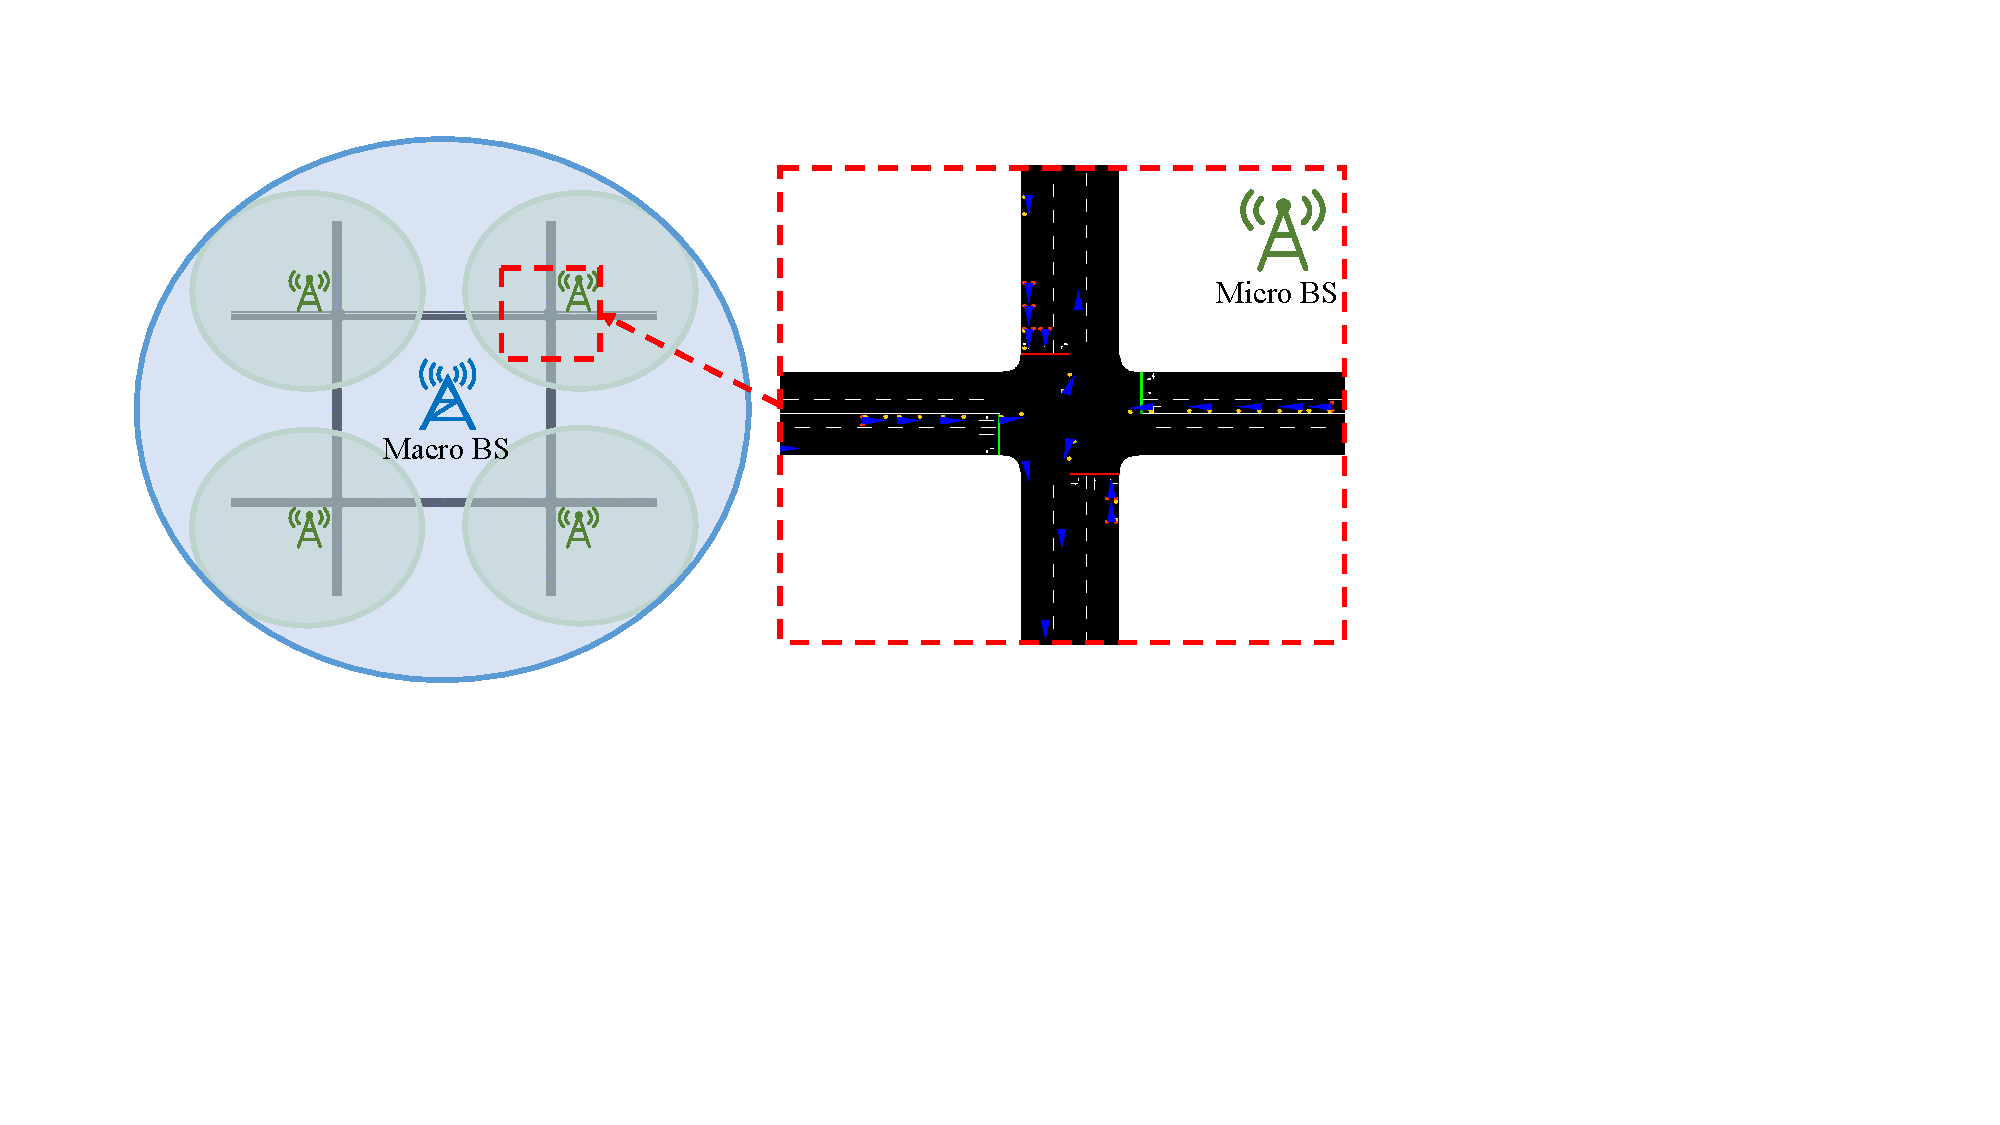
\includegraphics[width=0.45\textwidth, trim= 60 200 300 50,clip]{figures/system_model_v3.pdf}}
    \caption{The system model.}
    \label{fig:system_model}
    \end{figure}
\fi

We consider a vehicular communication scenario covered by a two-tier HetNet adopting a {control–data-plane separation} architecture. 
% omit for 13 pages
% as illustrated in Fig.~\ref{fig:system_model}
The network consists of one macro BS and $M$ micro BSs. The macro BS serves as the control-plane anchor and makes {frame-level} PHO decisions, while the micro BSs execute the corresponding {data-plane} re-association and perform {slot-level} BF and RA.
The BS set is denoted by $\mathcal{M} = \{0, 1, \dots, M\}$, where index $m=0$ represents the macro BS and $m>0$ represents a micro BS. BS-$m$ is allocated $K_m$ orthogonal RBs in the frequency band $f_m$, where each RB has a bandwidth of $B_m$ and a per-RB transmit power of $p_m$. 
For simplicity, all micro BSs are assumed to have identical frequency configurations, i.e., $K_m = K_\mu$, $f_m = f_\mu$ and $B_m = B_\mu$ for all $m>0$, while the macro BS has distinct parameters ${K_0, f_0, B_0}$.

We model the system in discrete time, indexed by slots $n \in \{0, 1, \dots\}$ of duration $\Delta t$. At any time slot $n$, the set of vehicles is $\mathcal{V}(n)$, with cardinality $V(n) = |\mathcal{V}(n)|$. The {data-plane}
connection between BS-$m$ and vehicle-$v \in \mathcal{V}(n)$ is represented by a binary indicator $u_{m,v}(n)$, where $u_{m,v}(n)=1$ signifies \currentdel{an active data-plane connection}\rev{the selected data-plane association} and $u_{m,v}(n)=0$ otherwise. Each vehicle can be associated with at most one BS on the data plane at a time, which imposes the constraint:
\begin{equation}
    \sum_{m=0}^{M} u_{m,v}(n) \leq 1, \quad \forall v \in \mathcal{V}(n).
    \label{eq:connection_cons}
\end{equation}
Note that the control-plane connection to the macro BS is always maintained and thus is not explicitly modeled.

The data-plane connection state $u_{m,v}(n)$ is managed by a central PHO server deployed at the macro BS and updated periodically over a time window of $N_{\rm HO}$ slots, which define a PHO frame. The handover configuration for the $x$-th frame is determined during the preceding $(x-1)$-th frame and remains static throughout frame~$x$. Therefore, we introduce a frame-based index. Let $\{\cdot\}^{[x]} \triangleq \{\cdot\}(xN_{\rm HO})$ denote a variable at the start of the $x$-th frame, and let $\{\cdot\}^{[x]}(i) \triangleq \{\cdot\}(xN_{\rm HO} + i)$ be the variable at the $i$-th slot within that frame, where $i \in \mathcal{N}_{\rm HO} \triangleq \{0,1,\dots,N_{\rm HO}-1\}$. Consequently, the connection state is constant within any frame, which is expressed as:
    \begin{equation}
        u_{m,v}^{[x]}(i) = u_{m,v}^{[x]}, \quad \forall i \in \mathcal{N}_{\rm HO}.
        \label{eq:PHO_cons}
    \end{equation}
We further assume the set of vehicles is static throughout each frame, denoted as $\mathcal{V}^{[x]}$.

\rev{After a PHO decision is made, the signaling exchanges required for HO preparation are assumed to finish before the current frame ends, without occupying data-service resources. A vehicle switching BS is assumed to experience a data-service interruption of duration $\tau_{\rm HO}=L_{\rm HO}\Delta t$ caused by HO execution at the start of the next frame, where $L_{\rm HO}$ is a nonnegative integer less than $N_{\rm HO}$. We assume successful HO execution for all PHO decisions. The macro control-plane connection and periodic CSI probing remain available during this data-plane HO interruption.}

\rev{Let $\delta_v^{[x]}=1$ if vehicle-$v$ changes its serving BS from frame-$(x-1)$ to frame-$x$, and $\delta_v^{[x]}=0$ otherwise. Its slot-level data-service availability is}
\begin{equation}
    \rev{s_v^{[x]}(i)=1-\delta_v^{[x]}\mathbf{1}\{i<L_{\rm HO}\},}
    \label{eq:HO_availability}
\end{equation}
\rev{where $\mathbf{1}\{\cdot\}$ is the indicator function.}

\subsection{Channel Model}

We specify the channel models used to calculate the instantaneous desired-link gains $g_{m,v}^{[x]}(i)$ for both macro-to-vehicle ($m=0$) and micro-to-vehicle ($m>0$) links, as well as the \currentdel{interference-link}\rev{interfering-link} gains when applicable.

\subsubsection{Channel model for macro BS}

\textcolor{black}{
The macro BS operates in a lower-frequency band (e.g., the microwave band) to provide wide-area coverage. 
}
The frame-averaged channel gain between the macro BS and vehicle-$v$ during the $x$-th frame, denoted as $G_{0,v}^{[x]}$, is modeled as
\begin{equation}
    G_{0,v}^{[x]} = \alpha \left(d_{0,v}^{[x]}\right)^{-\beta} 10^{S_v^{[x]}/10},
    \label{eq:avg channel gain}
\end{equation}
where $\alpha$ is a power gain factor, $\beta$ is the path loss exponent, and $d_{m,v}^{[x]}$ is the distance between BS-$m$ and vehicle-$v$ in the $x$-th frame. The term $S_v^{[x]}$ captures the shadow fading effect, which is modeled as an independent and identically distributed (i.i.d.) zero-mean Gaussian random variable with variance $\sigma_S^2$. 

Based on the frame-averaged channel gain $G_{0,v}^{[x]}$, the instantaneous channel gain $g_{0,v}^{[x]}(i)$ in the $i$-th time slot of the $x$-th frame is modeled by Rician fading as
\begin{equation}
    g_{0,v}^{[x]}(i) = G_{0,v}^{[x]}\left\|\sqrt{\frac{K_{\rm R}}{K_{\rm R}+1}} + \sqrt{\frac{1}{K_{\rm R}+1}} h_{0,v}^{[x]}(i)\right\|^2,
    \label{eq:instant channel condition}
\end{equation}
where $K_{\rm R}$ is the Rician K-factor and $h_{m,v}^{[x]}(i) \sim \mathcal{CN}\left(0,1\right)$ is an i.i.d. standard complex Gaussian random variable. 

\subsubsection{Channel model for micro BS}
\label{sec:micro_channel_model}
%In contrast, each micro BS utilizes a higher-frequency band (e.g., the mmWave band)  to take advantage of the large available bandwidth for high-capacity communications. To compensate for the more severe path loss at these frequencies, each micro BS is equipped with a uniform linear array (ULA) of $M_{\rm T}$ transmit antennas. Paired with the $M_{\rm R}$ receive antennas on each vehicle for the higher-frequency band, this configuration creates a multiple-input multiple-output (MIMO) link. 

\textcolor{black}{
Each micro BS operates in a higher-frequency band (e.g., the mmWave band) and is equipped with a uniform linear array (ULA) of $M_{\rm T}$ antennas, while each vehicle has $M_{\rm R}$ antennas at this band.
}
For the micro-to-vehicle links, we adopt a geometric stochastic MIMO channel model~\cite{molisch04}. The channel between micro BS-$m$ and vehicle-$v$ during the $x$-th frame is represented by the frame-averaged channel matrix $\boldsymbol{H}_{m,v}^{[x]} \in \mathbb{C}^{M_{\rm R} \times M_{\rm T}}$, which is modeled as a sum of $L$ distinct propagation paths:
\begin{equation}
\label{eq:MIMO_channel}
    \boldsymbol{H}_{m,v}^{[x]} = \sqrt{M_{\rm T} M_{\rm R}} \sum_{l=1}^{L} \gamma_{l} \boldsymbol{a}_{\rm R}(\theta_{l}) \boldsymbol{a}_{\rm T}(\psi_{l})^{\dagger},
\end{equation}
where $\gamma_l$, $\theta_l$, and $\psi_l$ denote the complex impulse response, angle of arrival (AoA), and angle of departure (AoD) of the $l$-th path, respectively. The vectors $\boldsymbol{a}_{\rm R}(\cdot) \in \mathbb{C}^{M_{\rm R}}$ and $\boldsymbol{a}_{\rm T}(\cdot) \in \mathbb{C}^{M_{\rm T}}$ are the receive and transmit array response vectors. For the ULAs, the array response vector is given by
\begin{equation}
    [\boldsymbol{a}(\phi)]_i = \frac{1}{\sqrt{N}} e^{-j \frac{2\pi d}{\lambda} i \sin\phi}, \quad i=0, \dots, N-1,
\end{equation}
where $N$ is the number of antennas ($M_{\rm T}$ or $M_{\rm R}$), $d$ is the inter-element spacing (typically $d=\lambda/2$), $\lambda$ is the carrier wavelength, and $\phi$ is the AoA or AoD ($\theta_l$ or $\psi_l$).
The instantaneous channel matrix in the $i$-th slot of frame-$x$ is modeled by applying small-scale Rician fading as
\begin{equation}
    \boldsymbol{H}_{m,v}^{[x]}(i)=\left(\sqrt{\frac{K_{\rm R}}{K_{\rm R}+1}} + \sqrt{\frac{1}{K_{\rm R}+1}} h_{m,v}^{[x]}(i)\right) \cdot \boldsymbol{H}_{m,v}^{[x]}.
    \label{eq:instantaneous channel matrix}
\end{equation}

Beamforming is employed for the MIMO links by selecting precoding and combining vectors from predefined codebooks. 
Specifically, we use discrete Fourier transform (DFT) codebooks. A DFT codebook of size $N$ consists of $N$ orthogonal vectors, $\mathcal{C} = \{\boldsymbol{c}_0, \boldsymbol{c}_1, \dots, \boldsymbol{c}_{N-1}\}$, where each codeword $\boldsymbol{c}_n \in \mathbb{C}^{N \times 1}$ corresponds to a spatial direction. The $i$-th element of the $n$-th codeword is
\begin{equation}
\label{eq:dft_codebook}
    [\boldsymbol{c}_n]_i = \frac{1}{\sqrt{N}} e^{-j \frac{2\pi ni}{N}}, \quad \forall n, i \in \{0, 1, \dots, N-1\}.
\end{equation}
The transmit codebook $\mathcal{C}_{\rm T}$ is a DFT codebook of size $M_{\rm T}$, and the receive codebook $\mathcal{C}_{\rm R}$ is a DFT codebook of size $M_{\rm R}$. 

When micro~BS-$m$ serves vehicle-$v$ in the $x$-th frame, it selects a transmit precoding vector ${\bm{w}_{\rm T}}_{m,v}^{[x]}(i) \in \mathcal{C}_{\rm T}$, and vehicle-$v$ selects a receive combining vector ${\bm{w}_{\rm R}}_{m,v}^{[x]}(i) \in \mathcal{C}_{\rm R}$. The resulting
instantaneous {desired-link} channel gain is
\begin{equation}
\label{eq:mimo_instant_gain}
    g_{m,v}^{[x]}(i) = \left| \left({\bm{w}_{\rm R}}_{m,v}^{[x]}(i)\right)^{\dagger} \boldsymbol{H}_{m,v}^{[x]}(i) {\bm{w}_{\rm T}}_{m,v}^{[x]} (i)\right|^2.
\end{equation}
\currentdel{For an interfering micro BS-$m$ that does not serve vehicle-$v$, we do not explicitly model its beam pattern toward vehicle-$v$. Instead, the corresponding interference-link channel gain is approximated by the Frobenius norm–based average gain of the MIMO channel matrix:}\rev{When another micro BS-$m'$ serves vehicle-$v'$, the interfering-link gain from BS-$m'$ to vehicle-$v$ is}
\ifshowdeletions
\begin{equation*}
    \currentdel{\ensuremath{g_{{\rm I},m,v}^{[x]}(i)\triangleq
    \frac{1}{M_{\rm T}M_{\rm R}}\bigl\|\boldsymbol H_{m,v}^{[x]}(i)\bigr\|_F^2,}}
\end{equation*}
\fi
{\color{revisioncolor}
\begin{equation}
\label{eq:mimo_instant_gain_interference}
    g_{{\rm I},m',v,v'}^{[x]}(i)
    = \left|\left({\bm{w}_{\rm R}}_{m,v}^{[x]}(i)\right)^{\dagger}
    \boldsymbol{H}_{m',v}^{[x]}(i){\bm{w}_{\rm T}}_{m',v'}^{[x]}(i)\right|^2.
\end{equation}
}
\currentdel{which provides a simple approximation of the effective interference power under random transmit and receive beam directions.}


\subsection{Resource Allocation Model}

Let $k_{m,v}^{[x]}(i) \in \{0,1,\dots,K_m\}$ denote the number of RBs allocated by BS-$m$ to vehicle-$v$ in the $i$-th time slot of the $x$-th frame. Since RBs can only be allocated to connected users\rev{ without HO interruption}, this variable must satisfy
\begin{equation}
    k_{m,v}^{[x]}(i) = u_{m,v}^{[x]}\rev{s_v^{[x]}(i)}k_{m,v}^{[x]}(i), \quad \forall i \in \mathcal{N}_{\rm HO}.
    \label{eq:resource allocation cons}
\end{equation}
Each BS employs orthogonal frequency-division multiple access (OFDMA). Accordingly, the number of RBs utilized by BS-$m$, $k_{m}^{[x]}(i)$, is constrained by its total RB capacity $K_m$:
\begin{equation}
    k_{m}^{[x]}(i) \triangleq \sum_{v\in\mathcal{V}^{[x]}} k_{m,v}^{[x]}(i) \leq K_m.
    \label{eq:RB cons}
\end{equation}
The instantaneous transmit power of BS-$m$ is then given by
\begin{equation}
    P_m^{[x]}(i) = p_m k_{m}^{[x]}(i).
    \label{eq:BS instant power cons}
\end{equation}
The time-averaged system transmit power is the sum of the average power of all BSs:
\begin{align}
    \bar{P} & = \sum_{m=0}^M \bar{P}_m =\lim_{X\to\infty}\frac{1}{X} \sum_{x=0}^{X-1}\rev{\frac{1}{N_{\rm HO}}}\sum_{i \in \mathcal{N}_{\rm HO}} \sum_{m=0}^MP_m^{[x]}(i) \nonumber \\
    &=\lim_{X\to\infty}\frac{1}{XN_{\rm HO}}\sum_{x=0}^{X-1}\sum_{i \in \mathcal{N}_{\rm HO}}  \sum_{v\in\mathcal{V}^{[x]}} \sum_{m=0}^M p_m  k_{m,v}^{[x]}(i).
    \label{eq:area timeavg power cons}
\end{align}

\currentdel{Given allocated RBs, the instantaneous signal to interference plus noise ratio (SINR) of the desired-link from BS-$m$ to vehicle-$v$ is given by}\rev{For a link with $k_{m,v}^{[x]}(i)>0$, the signal-to-interference-plus-noise ratio (SINR) is modeled as}
\begin{equation}
    \mathrm{SINR}_{m,v}^{[x]}(i) = \frac{p_{m,v}^{[x]}(i) g_{m,v}^{[x]}(i)}{F_{ m}N_0 W_{m,v}^{[x]}(i) + I_{m,v}^{[x]}(i) },
    \label{eq:SINR}
\end{equation}
where $p_{m,v}^{[x]}(i) = k_{m,v}^{[x]}(i) p_m$ is the power allocated to the vehicle, $W_{m,v}^{[x]}(i) = k_{m,v}^{[x]}(i) B_m$ is the allocated bandwidth, $N_0$ is the noise power spectral density, $F_{m}$ is the noise figure, and $I_{m,v}^{[x]}(i)$ is the inter-cell interference. For the macro BS, $I_{0,v}^{[x]}(i)=0$ since its frequency band is orthogonal to those of micro BSs. 
\currentdel{For each micro BS, since the OFDMA-based RB allocation across different BSs is assumed to be independent and uniformly random, the expected number of overlapping RBs between the set of RBs allocated by BS-$m$ to vehicle-$v$ and the set of RBs utilized by any interfering BS-$m'$ is $\frac{k_{m,v}^{[x]}(i) k_{m'}^{[x]}(i)}{K_\mu}$.}\rev{Given the allocated RB counts, each micro BS assigns mutually disjoint RB sets to its associated vehicles uniformly at random, independently of the other micro BSs. The expected number of overlapping RBs between links $(m,v)$ and $(m',v')$, with $m'\ne m$, is therefore $k_{m,v}^{[x]}(i)k_{m',v'}^{[x]}(i)/K_\mu$.}
Accordingly, \currentdel{the interference can be modeled as}\rev{the interference power averaged over the random RB assignments is given by}
\begin{equation}
    \begin{aligned}
        & I_{m,v}^{[x]}(i) \\
        & =
        \begin{cases}
            \displaystyle
            \currentdel{\ensuremath{\sum\limits_{m'\neq 0,m} g_{{\rm I},m',v}^{[x]}(i) \frac{k_{m,v}^{[x]}(i) k_{m'}^{[x]}(i)}{K_\mu} p_{m'}}}\rev{\frac{k_{m,v}^{[x]}(i)}{K_\mu}
            \sum\limits_{\substack{m'\neq 0,m\\v'\in\mathcal V^{[x]}}}
            p_{m'}k_{m',v'}^{[x]}(i)g_{{\rm I},m',v,v'}^{[x]}(i)}, & m>0, \\
            \displaystyle
            0, & m=0.
        \end{cases}
    \end{aligned}
    \label{eq:interference}
\end{equation}
%This formulation provides an average interference approximation, which captures the expected impact of frequency-domain resource overlap among adjacent BSs without requiring explicit RB-level coordination.
\currentdel{By substituting the expressions for power, bandwidth and interference, the SINR term simplifies to}\rev{Under this average interference approximation, the link SINR is approximated as}
\begin{equation}
    \begin{aligned}
        & \mathrm{SINR}_{m,v}^{[x]}(i) \\
        & = 
        \begin{cases}
            \displaystyle
            \frac{ p_m g_{m,v}^{[x]}(i)}
            {F_m N_0 B_m 
             + \sum\limits_{\substack{m'\neq 0,m\\\rev{v'\in\mathcal V^{[x]}}}}
               \currentdel{\ensuremath{\frac{k_{m'}^{[x]}(i)}{K_\mu}p_{m'}g_{{\rm I},m',v}^{[x]}(i)}}\rev{\frac{p_{m'}k_{m',v'}^{[x]}(i)}{K_\mu}
               g_{{\rm I},m',v,v'}^{[x]}(i)}}, 
            & m>0, \\[2ex]
            \displaystyle
            \frac{ p_m g_{m,v}^{[x]}(i)}{F_m N_0 B_m}, 
            & m=0.
        \end{cases}
    \end{aligned}
    \label{eq:SINR simplified}
\end{equation}
\currentdel{Based on the Shannon-Hartley theorem, the instantaneous achievable rate of this link is expressed as}\rev{The corresponding link rate is modeled using the Shannon formula as}
\begin{align}
    R_{m,v}^{[x]}(i) & = W_{m,v}^{[x]}(i) \log_2 \left( 1 + \mathrm{SINR}_{m,v}^{[x]}(i) \right).
    \label{eq:instantaneous link achievable rate}
\end{align}
\rev{When $k_{m,v}^{[x]}(i)=0$, no data are transmitted on the link, and thus $R_{m,v}^{[x]}(i)=0$.}
Considering the beam-searching overhead, the instantaneous receive rate of vehicle–$v$ is given by
\begin{equation}
    r_{v}^{[x]}(i) = \sum_{m=0}^M \bigl(1-\eta_{m,v}^{[x]}(i) \bigl)R_{m,v}^{[x]}(i),
    \label{eq:instantaneous veh receive rate}
\end{equation}
where $\eta_{m,v}^{[x]}(i) \in [0,1)$ represents the throughput loss factor resulting from beam alignment. Specifically,
\begin{align}
\eta_{m,v}^{[x]}(i) = \eta N_{m,v}^{[x]}(i),
\end{align}
with $N_{m,v}^{[x]}(i)$ denoting the number of beam-search attempts conducted by BS–$m$ and vehicle–$v$ in the $i$-th slot of frame-$x$, and $\eta$ \currentdel{representing the ratio of OFDM symbols consumed by once beam search to the total number of OFDM symbols per slot}\rev{denoting the fraction of OFDM symbols in a slot required to probe one beam pair.}.
Besides, the frame-averaged receive rate of vehicle-$v$ is 
\begin{equation}
    \bar{r}_v^{[x]} \triangleq  \frac{1}{N_{\rm HO}}\sum_{ i \in \mathcal{N}_{\rm HO}}r_{v}^{[x]}(i),
    \label{eq:frame-averaged veh receive rate}
\end{equation}


\subsection{Traffic Model}
We model the data traffic for each vehicle-$v$ with a backlog queue, where $q_v(n)$ denotes its length at the beginning of time slot $n$. The queue length evolves as
\begin{equation}
    q_v(n+1) = \max \left\{ q_v(n) - r_v(n) \Delta t, 0 \right\} + a_v(n),
    \label{eq: queue update}
\end{equation}
where $a_v(n)$ is the amount of data arriving for vehicle-$v$ during time slot-$n$.
This model assumes that the existing backlog $q_v(n)$ is served first at a rate of $r_v(n)$, and new arrivals $a_v(n)$ are enqueued for service in subsequent slots. 
We denote the average data arrival rate for vehicle-$v$ as $\lambda_v$, thus we have $\mathbb{E}\left[ a_v(n) \right] = \lambda_v \Delta t$.
\rev{We consider Poisson arrivals that are independent across vehicles and slots, with $a_v(n)\sim\mathrm{Poisson} (\lambda_v\Delta t)$. This model does not capture temporally correlated traffic bursts.}

\currentdel{According to}\rev{\rev{Queueing delay is an important component of end-to-end latency, alongside transmission, propagation, and processing delays. We focus on queueing delay to assess how HO, BF, and RA jointly affect traffic accumulation through the available service rates.} Motivated by} \textit{Little's law} \cite{little1961proof}, \currentdel{the queuing latency $\tau_v(n)\approx \lambda_v^{-1}q_v(n)$}\rev{we define $\tau_v(n)\triangleq\lambda_v^{-1}q_v(n)$ as a queueing-delay proxy}. \currentdel{To keep $\tau_v(n)$ no more than a latency threshold $\tau_{\rm th}$, the queue length should satisfy the following latency constraint}\rev{Requiring this proxy not to exceed the latency threshold $\tau_v^{\rm th}$ of  vehicle-$v$  gives the queue-length-based latency constraint}:
\begin{equation}
    q_v(n) \leq \lambda_v \text{\currentdel{$\tau^{{\rm th}}$}}\rev{\tau_v^{\rm th}}.
    \label{eq:queue length cons}
\end{equation}

To evaluate the system performance with respect to this latency constraint, we define the latency constraint violation probability $U$ following the approach in \cite{kien17} as:
\begin{equation}
    U = \lim_{N\rightarrow\infty}\frac{1}{N}\sum_{n=0}^{N-1}  \frac{\sum_{v\in\mathcal{V}(n)}U_v(n)}{V(n)},
    \label{eq:violation probability}
\end{equation}
where $U_v(n) = 1$ if $q_v(n) > \lambda_v \text{\currentdel{$\tau^{{\rm th}}$}}\rev{\tau_v^{\rm th}}$, and $U_v(n) = 0$ otherwise. \currentdel{This metric serves as a measure of the system latency reliability.}\rev{Specifically, $U$ measures the probability that the queueing-delay proxy $\tau_v(n)$ exceeds its threshold $\tau_v^{\rm th}$.}


\section{Problem Formulation}{\label{sec:Problem Formulation}}

Our goal is to minimize the long-term system transmit power while satisfying the latency-constrained QoS requirements for all vehicles. This joint optimization of HO, BF and RA over different time scales is formulated as the following problem 
\begin{equation}
    \label{prob1}
    \begin{aligned}
        \textbf{P1:} \qquad  \min_{\bm{u},\bm{k}, \bm{\mathcal{W}}} & \bar{P} \\
        \textup{s.t.} \quad 
        \textup{C1}: \quad & q_v^{[x]}(i) \leq \lambda_v \text{\currentdel{$\tau^{{\rm th}}$}}\rev{\tau_v^{\rm th}}, \\
        \textup{C2}: \quad & \sum_{m=0}^{M} u_{m,v}^{[x]} \leq 1, \\
        \textup{C3}: \quad & \sum_{v\in\mathcal{V}^{[x]}} k_{m,v}^{[x]}(i) \leq K_m, \\
        \textup{C4}: \quad & k_{m,v}^{[x]}(i) = u_{m,v}^{[x]}\rev{s_v^{[x]}(i)}k_{m,v}^{[x]}(i), \\
        \textup{C5}: \quad & u_{m,v}^{[x]} \in \{0,1\}, \\
        \textup{C6}: \quad & k_{m,v}^{[x]}(i) \in \{0,1,\dots,K_m\}, \\
        \textup{C7}: \quad & {\bm{w}_{\rm T}}_{m,v}^{[x]}(i) \in \mathcal{C}_{\rm T}, \, {\bm{w}_{\rm R}}_{m,v}^{[x]}(i) \in \mathcal{C}_{\rm R}.
    \end{aligned}
\end{equation}
In \textbf{P1}, the decision variables are the sets of data-plane connection states $\bm{u} \triangleq \{ u_{m,v}^{[x]} \}$, RB allocation numbers $\bm{k} \triangleq \{ k_{m,v}^{[x]}(i) \}$, and BF vectors $\bm{\mathcal{W}} \triangleq \{ [{\bm{w}_{\rm T}}_{m,v}^{[x]}(i), {\bm{w}_{\rm R}}_{m,v}^{[x]}(i)] \}$. 
In our system, $\bm{u}$ is decided per frame, while $\bm{k}$ and $\bm{\mathcal{W}}$ are decided per time slot.
They are subject to several constraints. 
{C1} is the queue-length-based latency constraint equivalent to Eq.\eqref{eq:queue length cons}. 
The HO constraints {C2} and {C5} enforce that each vehicle connects to at most one BS in the data-plane. 
The RA constraints {C3}, {C4}, and {C6} limit the total RBs per BS, ensure RBs are only assigned to connected vehicles\rev{ without HO interruption}, and define the integer nature of $k_{m,v}^{[x]}(i)$. 
Finally, {C7} restricts the BF vectors to be chosen from the predefined finite codebooks, which makes the BF decision a combinatorial integer optimization component.

\textbf{P1} is a two-timescale SINLP. Obtaining its optimal \emph{online} solution is computationally prohibitive due to the following challenges:
\begin{enumerate}[label=\arabic*.]
    \item \textbf{Stochastic and causally observed dynamics}: 
    Future system states, including the vehicle set $\mathcal{V}^{[x]}$, the channel matrices $\boldsymbol{H}_{m,v}^{[x]}(i)$, and the traffic arrivals $a_v(n)$, are time-varying and only causally observable. Moreover, current decisions have lasting impacts on future power consumption and latency performance. Therefore, the long-horizon online optimization of \textbf{P1} is fundamentally challenging.
    \item \textbf{Combinatorial decision space and NP-hardness}: 
    All decision variables in \textbf{P1} are discrete and jointly define a high-dimensional decision space over BS-vehicle association, beam-pair selection, and RB allocation, further complicated by inter-cell interference coupling through the SINR expressions. Consequently, \textbf{P1} is an NP-hard integer nonconvex optimization problem whose feasible set grows exponentially with the numbers of BSs, vehicles, RBs, and BF codebook sizes, rendering exhaustive search or exact global optimization impractical.    
    \item \textbf{Coupled two-timescale optimization}: 
    Frame-level HO decisions determine the association topology and constrain the slot-level BF and RA decisions within that frame, while the chosen BF vectors directly affect the desired-link gains, thereby influencing RB allocation and queue evolution. Such cross-timescale dependencies imply that optimizing PHO, BF, and RA in isolation can lead to persistently suboptimal performance, and call for low-complexity joint coordination mechanisms.
    \item \textbf{Prohibitive CSI measurement overhead}: 
    An online global optimizer would require timely and accurate per-link CSI for all BS-vehicle links and beam-pair options to evaluate channel gains and interference. 
    In high-mobility vehicular scenarios, acquiring such per-link CSI via frequent channel measurements, beam training, and feedback incurs excessive overhead and latency, thus impractical for realization.
\end{enumerate}

In summary, the NP-hardness of \textbf{P1}, together with stochastic dynamics, two-timescale coupling, and the prohibitive overhead of real-time per-link CSI acquisition, makes the online global optimization for \textbf{P1} computationally prohibitive.


\section{Algorithm Design}
\label{sec:Algorithm Design}

To solve \textbf{P1} with an efficient and computationally feasible online approach, we propose a novel algorithm framework named {M}achine-learning-based {E}nergy-{E}fficient proac{T}ive COBRA ({MEET-COBRA}). 
It leverages ML-predicted beam-pair candidates and channel gains to enable proactive, two-timescale COBRA optimization\currentdel{: the}\rev{. The} central PHO server determines the next-frame PHO configuration globally, while each BS performs slot-level BF and RA locally to serve its associated vehicles. 
The following subsections introduce the ML-based prediction module, the \emph{predictive, frame-level} PHO algorithm, the \emph{real-time, slot-level} BF and RA algorithms, and the overall MEET-COBRA procedure.

\subsection{ML-Based Prediction}{\label{subsection: ML pred}}

\begin{figure}
\centerline{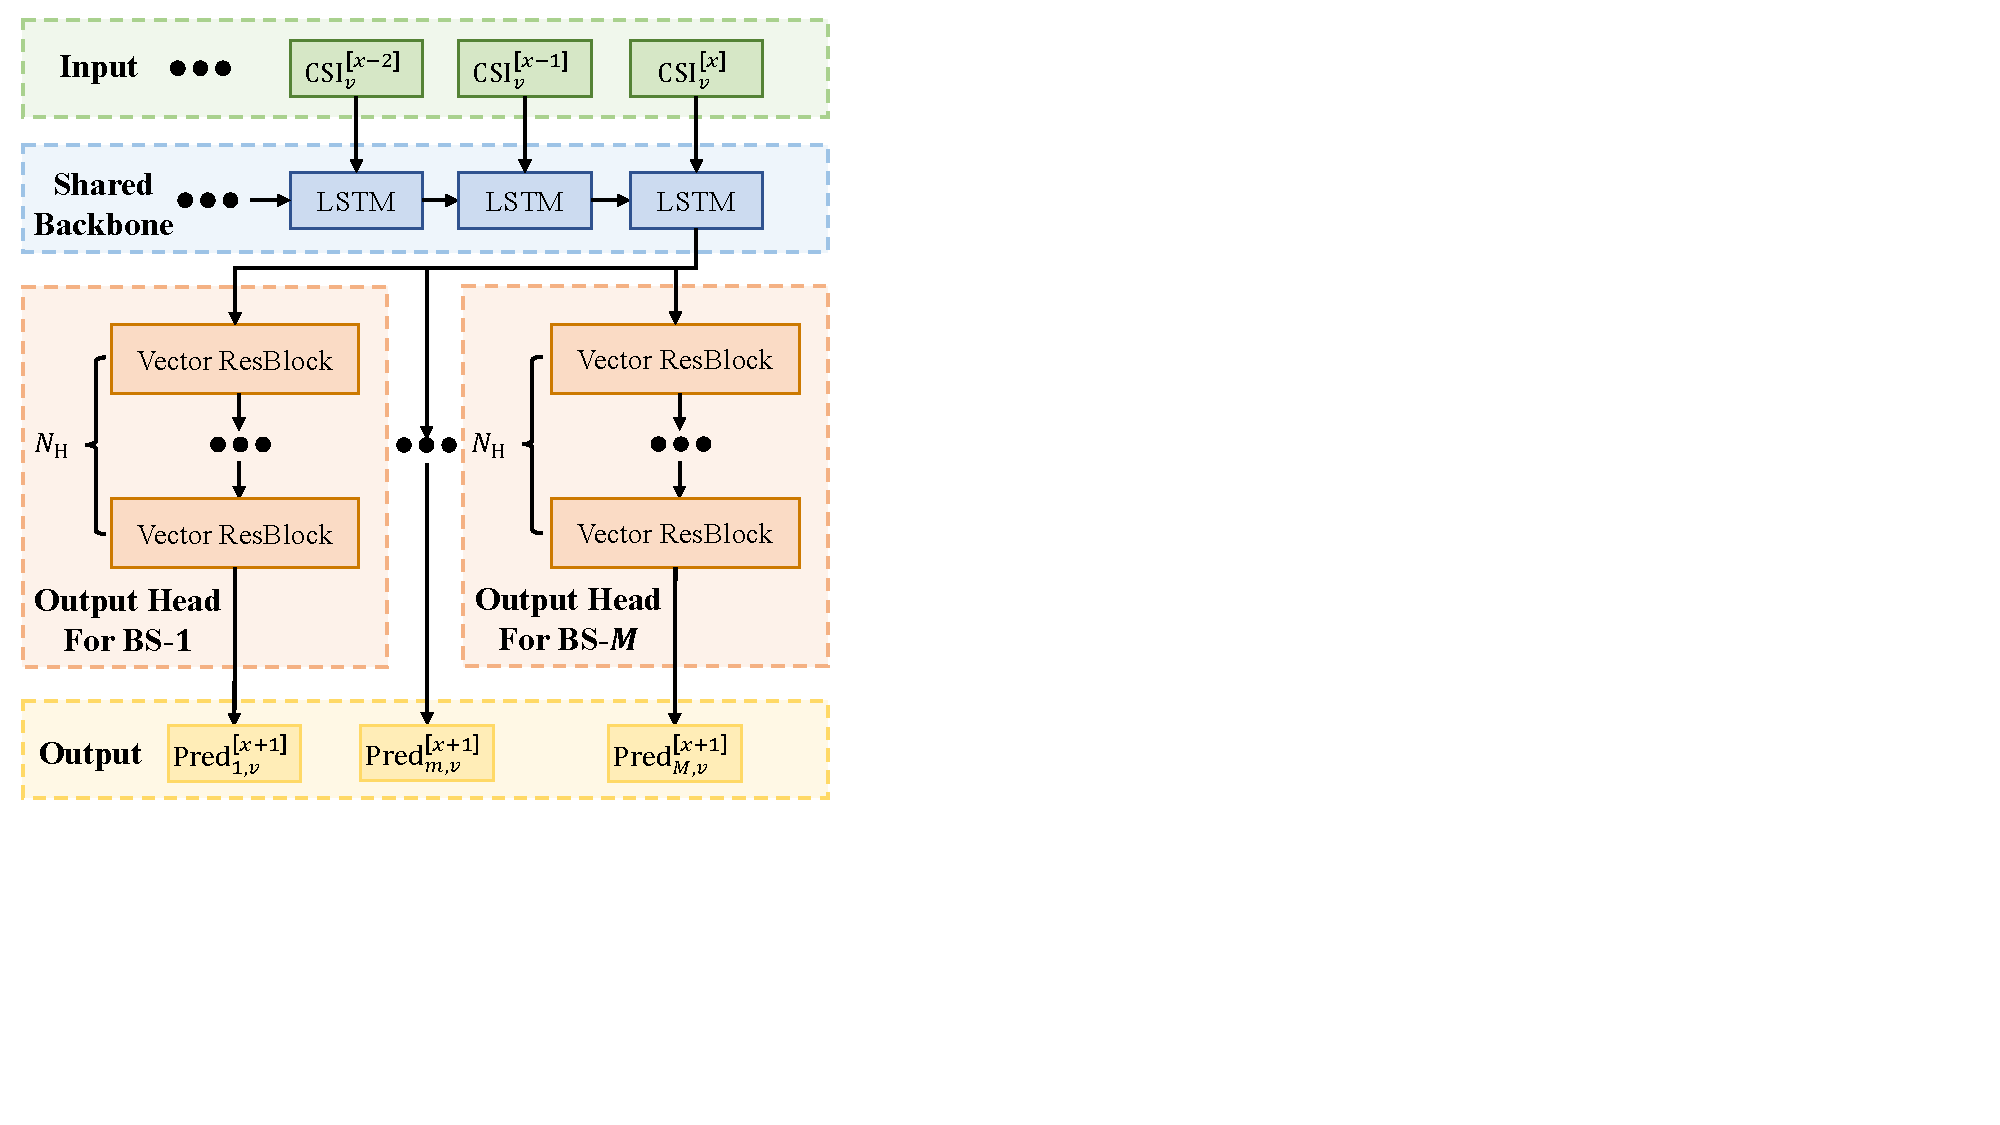
\includegraphics[width=0.5\textwidth, trim= 0 150 550 0,clip]{figures/NNmodel.pdf}}
\caption{\currentdel{The architecture of the proposed neural network model for the optimal beam-pair and channel-gain prediction.}\rev{Neural network architecture for predicting the next-frame best beam-pair index, its corresponding desired-link gain, and the interfering-link gain.}}
\label{fig:NN model}
\end{figure}

A neural network (NN) model is developed to predict, for each vehicle, the next-frame \currentdel{optimal beam-pairs, desired-link gains}\rev{best beam-pair indices, their corresponding desired-link gains}, and \currentdel{interference-link}\rev{interfering-link} gains to all micro BSs. To reduce CSI feedback overhead and avoid centralized NN inference latency that grows with the number of vehicles, each vehicle performs NN inference locally based on its historical CSI measurements obtained from a low-overhead pilot probing procedure, and reports only the prediction results to the macro BS.
The site-specific NN model is shared among vehicles by the macro BS over the control channel.
\rev{Deployment in a different propagation environment or BS layout requires retraining the prediction models using channel data from the target site.}
As shown in Fig.~\ref{fig:NN model}, the NN consists of an input preprocessing layer, a shared feature-extraction backbone, and $M$ micro-BS-specific output heads.

\subsubsection{Input Layer}

The NN input is a sequence of historical CSI measurements of vehicle-$v$. In each frame, the CSI is measured by a low-overhead pilot probing mechanism based on \emph{pilot superposition}.
Specifically, at the beginning of frame-$x$, all micro BSs simultaneously transmit a series of $N_{\rm P}$ pilot beams uniformly selected from the transmit codebook $\mathcal{C}_{\rm T}$. 
In the $p$-th pilot probing ($p=1,\dots,N_{\rm P}$), the received signal at vehicle-$v$ is the superposition of pilots from all micro BSs, i.e.,
\begin{equation}
\label{eq:pilot_superposition}
    \bm{y}_{v}^{[x]}(p)
    =
    \sum_{m=1}^{M} \boldsymbol{H}_{m,v}^{[x]} \bm{w}_{{\rm T},m}(p)\, s(p)
    + \bm{n}_{v}^{[x]}(p),
\end{equation}
where $\bm{w}_{{\rm T},m}(p)\in\mathcal{C}_{\rm T}$ is the transmit beam used by micro BS-$m$ in the $p$-th probing, $s(p)$ is the pilot symbol, and $\bm{n}_{v}^{[x]}(p)$ is the received noise.
Compared with exhaustive per-BS per-beam pilot sweeping with overhead $O(MM_{\rm T})$, pilot superposition reduces the measurement overhead to $O(N_{\rm P})$.
Accordingly, the CSI measured by vehicle-$v$ in frame-$x$ is defined as
\begin{equation}
\label{eq:CSI_stack}
    {\rm CSI}_v^{[x]} \triangleq 
    \big[ \bm{y}_{v}^{[x]}(1)^{\mathsf T},\ \bm{y}_{v}^{[x]}(2)^{\mathsf T},\ \dots,\ \bm{y}_{v}^{[x]}(N_{\rm P})^{\mathsf T} \big]^{\mathsf T}
    \in \mathbb{C}^{M_{\rm R}N_{\rm P}},
\end{equation}
where $\bm{y}_{v}^{[x]}(p)\in\mathbb{C}^{M_{\rm R}}$ is given in \eqref{eq:pilot_superposition}.
Before being fed into the NN, ${\rm CSI}_v^{[x]}$ is converted to a real-valued feature vector by normalizing amplitudes (in dB) and phases, and concatenating them as $\bm{z}_{\text{in},v}^{[x]} \in \mathbb{R}^{2M_{\rm R}N_{\rm P}}$. This preprocessing operation is denoted as $f_{\text{prep}}$:
\begin{equation}
\label{eq:preprocess_CSI}
    \bm{z}_{\text{in},v}^{[x]} = f_{\text{prep}} \left({\rm CSI}_v^{[x]} \right).
\end{equation}


\subsubsection{Shared Backbone}

The shared backbone processes the historical CSI sequence of each vehicle to extract a compact representation of its mobility pattern and surrounding radio environment. It consists of a Long Short-Term Memory (LSTM) unit~\cite{lstm}. 
The LSTM unit, with $N_{\rm C}$ hidden cells, captures the temporal dependencies in the CSI by maintaining a hidden state $\bm{h}_v \in \mathbb{R}^{N_{\rm C}}$ and a cell state $\bm{c}_v \in \mathbb{R}^{N_{\rm C}}$. In frame-$x$, the LSTM unit updates these states based on the current CSI feature vector $\bm{z}_{\text{in},v}^{[x]}$ and the previous states $(\bm{h}_v^{[x-1]}, \bm{c}_v^{[x-1]})$:
\begin{equation}
\label{eq:lstm_update}
    \left(\bm{h}_v^{[x]}, \bm{c}_v^{[x]}\right) = f_{\text{LSTM}} \left(\bm{z}_{\text{in},v}^{[x]}, \bm{h}_v^{[x-1]}, \bm{c}_v^{[x-1]} ;\bm{\theta}_{\text{LSTM}} \right),
\end{equation}
where $f_{\text{LSTM}}$ denotes the LSTM transformations and $\bm{\theta}_{\text{LSTM}}$ denotes the corresponding weights. 
\rev{The states are retained across frames for each vehicle, so online inference processes only the current CSI feature vector.}
% omit for 13 pages
\iffalse
    \begin{remark}
    This stateful update in \eqref{eq:lstm_update} enables the NN model to summarize historical CSI without reprocessing the entire CSI history in every frame, thus reducing computational overhead.
    \end{remark}
\fi

\subsubsection{Per-BS Output Heads}
The backbone hidden state $\bm{h}_v^{[x]}$ is fed into $M$ micro-BS-specific output heads, one for each micro BS:
\begin{equation}
\label{eq:OutputHead}
    \text{Pred}_{m,v}^{[x+1]} = f_{\text{hd}} \left(\bm{h}_v^{[x]};\bm{\theta}_{\text{hd},m} \right), \, \forall m \in \{1,2,\dots,M\},
\end{equation}
where $f_{\text{hd}}$ represents the common head structure, 
$\bm{\theta}_{\text{hd},m}$ denotes the weights of the $m$-th head, and $\text{Pred}_{m,v}^{[x+1]}$ is the prediction for the link between micro BS-$m$ and vehicle-$v$ in frame-$(x\!+\!1)$.
Each head comprises $N_{\rm H}$ stacked vector ResBlock units~\cite{He2016} with feature dimension $N_{\rm C}$, followed by a task-specific final layer. For beam-pair prediction, the final layer has dimension $M_{\rm T}M_{\rm R}$, whereas for channel-gain prediction it has dimension~1.



\subsubsection{Output Prediction}

\currentdel{Although the beam-pair and channel-gain prediction share the same NN architecture, they are implemented as distinct models with independently trained weights:}\rev{Beam-pair and channel-gain prediction are implemented using independently trained NN models with a common backbone architecture and task-specific output layers:}
\begin{enumerate}[label=\arabic*.]
    \item \textbf{Beam Prediction Model}: \currentdel{The optimal beam-pair}\rev{Beam-pair} prediction is formulated as a multi-class classification task. The final layer of each output head employs a softmax activation function to generate a predicted probability distribution $\Tilde{\mathcal{P}}_{m,v}^{[x+1]}$ over the $M_{\rm T}M_{\rm R}$ \currentdel{beam-pairs}\rev{beam pairs}.
    The model is trained with a cross-entropy loss, using a one-hot label whose non-zero entry indicates the index of the optimal \currentdel{beam-pair}\rev{beam pair} that
    maximizes the \rev{frame-averaged }desired-link gain in \currentdel{frame-}\rev{frame~}$(x\!+\!1)$.
    
    \item \textbf{Gain Prediction Models}: \currentdel{The channel-gain prediction is regarded as a regression task. For each micro BS–vehicle pair-$(m,v)$, we train two separate NN models with identical architecture but independent weights: one for the optimal desired-link gain and one for the interference-link gain.}\rev{Channel-gain prediction is formulated as a regression task. We train two separate NN models with the same architecture but independent weights, one for the optimal desired-link gain and the other for the beam-averaged interfering-link gain. Each model has one output head per micro BS.}
    In the desired-link \rev{gain }model, each head outputs a scalar $\Tilde{G}_{m,v}^{[x+1]}$ to approximate the \currentdel{frame-averaged optimal}\rev{maximum frame-averaged} desired-link gain
    \begin{equation}
        G_{{\rm opt},m,v}^{[x+1]}
        \triangleq
        \max_{{\bm{w}_{\rm T}}_{m,v}^{[x+1]},
              {\bm{w}_{\rm R}}_{m,v}^{[x+1]}} G_{m,v}^{[x+1]},
    \end{equation}
    where $G_{m,v}^{[x+1]}$ is obtained by averaging the instantaneous desired-link gains in Eq. \eqref{eq:mimo_instant_gain} over all slots in frame~$(x\!+\!1)$.
    \currentdel{The interference-link model is similarly defined: its final layer outputs a scalar $\Tilde{G}_{{\rm I},m,v}^{[x+1]}$ with label $G_{{\rm I},m,v}^{[x+1]}$, given by the frame-average of the instantaneous interference-link gains in Eq. \mbox{\eqref{eq:mimo_instant_gain_interference}}.}\rev{The interfering-link gain in~\eqref{eq:mimo_instant_gain_interference} depends on the receive beam of the desired link and the transmit beam used by the interfering BS. To obtain a prediction target independent of these beam selections, we adopt the beam-averaged surrogate}
    {\color{revisioncolor}
    \begin{equation}
        \label{eq:mimo_average_gain_interference}
        \tilde{g}_{{\rm I},m',v}^{[x]}(i)
        \triangleq \frac{1}{M_{\rm T}M_{\rm R}}
        \bigl\|\boldsymbol H_{m',v}^{[x]}(i)\bigr\|_F^2,
    \end{equation}
    }\rev{which equals the effective gain uniformly averaged over all beam pairs in the transmit and receive DFT codebooks. Each head of the interfering-link gain model outputs $\Tilde{G}_{{\rm I},m',v}^{[x+1]}$, with training label $G_{{\rm I},m',v}^{[x+1]}$ defined as the frame average of $\tilde{g}_{{\rm I},m',v}^{[x+1]}(i)$.}
    % Beam-average labels and the retrained predictor are verified in
    % experiment/revision_fig4_update_20260922_report.md.
    Both models are trained using a mean \currentdel{square}\rev{squared} error (MSE) loss function, with predictions and labels represented in normalized dB.
\end{enumerate}

\currentdel{The predictions $\bigl\{\Tilde{\mathcal{P}}_{m,v}^{[x+1]}, \Tilde{G}_{m,v}^{[x+1]}, \Tilde{G}_{{\rm I},m,v}^{[x+1]}\bigr\}_{m=1}^M$ reported by each vehicle-$v$ to the macro BS serve as key inputs to the subsequent PHO and BF stages.}For the macro BS ($m=0$), whose low-frequency link does not involve beam alignment or inter-cell interference, only the frame-averaged desired-link gain $\Tilde{G}_{0,v}^{[x+1]}$ is required. Owing to the slow variation of the macro-channel, this gain is approximated by the channel gain estimated from control-plane measurements in the current frame, without NN-based prediction.

\subsection{Generalized Assignment-based Proactive Handover}
\label{subsection:PHO strategy}

This subsection proposes a generalized assignment-based proactive handover (GAP-HO) algorithm, detailed in Alg.~\ref{alg:GAP-HO}, which determines the data-plane connection state for the upcoming frame. Its primary objective is to minimize the per-frame HetNet transmit power while satisfying both the latency-constrained QoS requirements of vehicles and the RB-capacity constraints of BSs.

To ensure queue stability, the expected frame-averaged receive rate $\mathbb{E}[\bar{r}_v^{[x]}]$ should be no less than the data arrival rate $\lambda_v$. The following theorem establishes a lower bound on the frame-averaged number of RBs required to satisfy this condition in the interference-free case.


\begin{theorem}
\label{theorem:1}
Consider vehicle-$v$ associated with BS-$m$ in the $x$-th frame. Given
$G_{m,v}^{[x]}$, $\lambda_v$, $B_m$, $p_m$, $F_m$ and $N_0$, the frame-averaged
number of allocated RBs, denoted by $\bar{k}_{m,v}^{[x]}$, required to ensure
$\mathbb{E}[\bar{r}_v^{[x]}] \geq \lambda_v$ satisfies
\begin{equation}
   \label{eq:theorem1}
   \bar{k}_{m,v}^{[x]} \geq
   \lambda_v \Bigl[ B_m \log_2 \Bigl( 1 + \frac{ p_m G_{m,v}^{[x]}}
   {F_m N_0 B_m} \Bigr) \Bigr]^{-1},
\end{equation}
where
$\bar{k}_{m,v}^{[x]} \triangleq N_{\rm HO}^{-1} \sum_{ i \in \mathcal{N}_{\rm HO}} k_{m,v}^{[x]}(i)$.
\end{theorem}
\begin{proof}
Since vehicle-$v$ is associated with BS-$m$ in frame-$x$, we have $u_{m,v}^{[x]}=1$ and $u_{m',v}^{[x]}=0$ for all $m'\neq m$. Combining
\eqref{eq:resource allocation cons},
\eqref{eq:instantaneous link achievable rate},
\eqref{eq:instantaneous veh receive rate}, and
\eqref{eq:frame-averaged veh receive rate}, the frame-averaged receive rate is
\begin{equation}
    \bar{r}_v^{[x]}
    = \frac{1}{N_{\rm HO}}\sum_{i \in \mathcal{N}_{\rm HO}}
      k_{m,v}^{[x]}(i) B_m
      \log_2\!\left(1 + \frac{p_m g_{m,v}^{[x]}(i)}{F_m N_0 B_m}\right).
\end{equation}

For any constant $C>0$, the function $f(z)=\log_2(1+Cz)$ is concave on $z>0$.
By Jensen's inequality,
\begin{equation}
\label{eq:Jensen Inequality}
    \mathbb{E}\!\left[
      \log_2\!\left(1 + \frac{p_m g_{m,v}^{[x]}(i)}{F_m N_0 B_m}\right)
    \right]
    \leq
    \log_2\!\left(1 + \frac{p_m \mathbb{E}[g_{m,v}^{[x]}(i)]}{F_m N_0 B_m}\right).
\end{equation}
Moreover, by \eqref{eq:mimo_instant_gain}, $\mathbb{E}[g_{m,v}^{[x]}(i)] =
G_{m,v}^{[x]}$. Taking expectation of $\bar{r}_v^{[x]}$ and using
\eqref{eq:Jensen Inequality} yield
\begin{align}
    \mathbb{E}[\bar{r}_v^{[x]}]
    &=
    \frac{1}{N_{\rm HO}} \sum_{i \in \mathcal{N}_{\rm HO}}
    k_{m,v}^{[x]}(i) B_m
    \mathbb{E}\!\left[
      \log_2\!\left(1 + \frac{p_m g_{m,v}^{[x]}(i)}{F_m N_0 B_m}\right)
    \right] \nonumber\\
    &\leq
    \frac{1}{N_{\rm HO}} \sum_{i \in \mathcal{N}_{\rm HO}}
    k_{m,v}^{[x]}(i) B_m
    \log_2\!\left(1 + \frac{p_m G_{m,v}^{[x]}}{F_m N_0 B_m}\right) \nonumber\\
    &= \bar{k}_{m,v}^{[x]} B_m
       \log_2\!\left(1 + \frac{p_m G_{m,v}^{[x]}}{F_m N_0 B_m}\right).
\end{align}
Combining with $\mathbb{E}[\bar{r}_v^{[x]}] \geq \lambda_v$, we obtain the lower bound in \eqref{eq:theorem1}. This completes the proof.
\end{proof}

Based on Theorem~\ref{theorem:1}, we now construct frame-averaged RB-demand estimates for each BS–vehicle pair-$(m,v)$ in frame-$(x\!+\!1)$.
For the macro BS ($m=0$), whose low-frequency link is free of inter-cell interference and beam-alignment overhead, the required frame-averaged number of RBs for vehicle-$v$ is estimated as 
\begin{equation}
\label{eq:RB_demand_hat_macro}
    \Tilde{k}_{0,v}^{[x+1]}
    = \lambda_v
      \Bigl[
        B_0 \log_2 \Bigl(
        1 + \frac{ p_0 \Tilde{G}_{0,v}^{[x+1]}}{F_0 N_0 B_0}
        \Bigr)
      \Bigr]^{-1},
\end{equation}
where $\Tilde{G}_{0,v}^{[x+1]}$ is estimated from control-plane measurements in the current frame.

For each micro BS ($m>0$), the lower bound in Theorem~\ref{theorem:1} is extended to account for inter-cell interference and beam-alignment overhead, while enhancing robustness against occasional large NN prediction errors. \currentdel{Given the NN-predicted frame-averaged gains}\rev{Given the NN predictions of the frame-averaged desired-link gains and interfering-link gain surrogates} for frame-$(x\!+\!1)$, each gain is smoothed by weighted averaging with the corresponding gain measured in frame-$x$ (when available); if no measurement exists, the NN prediction is used directly. With a slight abuse of notation, we still denote these robustness-enhanced gain estimates by $\Tilde{G}_{m,v}^{[x+1]}$ and $\Tilde{G}_{{\rm I},m',v}^{[x+1]}$. The effective SINR for vehicle-$v$ served by BS-$m$ in frame-$(x\!+\!1)$ is then approximated as
\begin{equation}
\label{eq:eff_SINR_hat}
    \widetilde{\mathrm{SINR}}_{m,v}^{[x+1]}
    = \frac{p_m \Tilde{G}_{m,v}^{[x+1]}}
           {F_m N_0 B_m
            + \sum\limits_{m'\neq 0,m}
              \frac{\Tilde{k}_{m'}^{[x+1]}}{K_\mu}\, p_{m'} \Tilde{G}_{{\rm I},m',v}^{[x+1]}},
\end{equation}
where $\Tilde{k}_{m'}^{[x+1]}$ denotes the estimated frame-averaged RB usage of BS-$m'$ in frame-$(x\!+\!1)$ and $K_\mu$ is the RB capacity of each micro BS. To capture the beam-training overhead, we conservatively assume that at most $M_{\rm P}$ beam-search attempts are performed per slot, so that the effective data-transmission fraction per slot is\rev{ at least} $(1-\eta M_{\rm P})$. Therefore, a conservative estimate of the required frame-averaged number of RBs is
\begin{equation}
\label{eq:RB_demand_hat}
    \Tilde{k}_{m,v}^{[x+1]}
    = \frac{\lambda_v}{(1-\eta M_{\rm P}) B_m \log_2\!\bigl(1+\widetilde{\mathrm{SINR}}_{m,v}^{[x+1]}\bigr)},
    \quad m>0.
\end{equation}

\begin{algorithm}[htbp]
    \caption{Generalized Assignment-based Proactive Handover (GAP-HO)}
    \label{alg:GAP-HO}
    \renewcommand{\algorithmicrequire}{\textbf{Input:}}
    \renewcommand{\algorithmicensure}{\textbf{Output:}}
    \begin{algorithmic}[1]
        \REQUIRE
        $\Tilde{G}_{m,v}^{[x+1]}, \Tilde{G}_{{\rm I},m,v}^{[x+1]}, \lambda_v, p_m, B_m, F_m, K_m, N_0, K_\mu, N_{\rm iter}$, $M_{\rm P}, \eta, \zeta$\currentdel{$, \epsilon$}\rev{, $u_{m,v}^{[x]}, L_{\rm HO}, N_{\rm HO}$};
        \ENSURE
        $u_{m,v}^{[x+1]}$;

        \STATE \textbf{Initialize} $\Tilde{k}_{m}^{[x+1]} \gets K_\mu$ for all $m>0$;
        \STATE \rev{Compute $c_{m,v}^{[x+1]}$ for all $m \in \mathcal{M}$ and $v \in \mathcal{V}^{[x]}$ by \eqref{eq:HO_capacity_factor};}

        \STATE Compute $\Tilde{k}_{0,v}^{[x+1]}$ for all $v \in \mathcal{V}^{[x]}$
        by \eqref{eq:RB_demand_hat_macro};

        \FOR{$n_{\rm iter} = 1$ to $N_{\rm iter}$}
            \STATE Compute $\Tilde{k}_{m,v}^{[x+1]}$ for each $m>0$ and $v \in \mathcal{V}^{[x]}$ by \eqref{eq:RB_demand_hat};

            \STATE Form \textbf{P2} with $\{\Tilde{k}_{m,v}^{[x+1]}\}$\rev{ and $\{c_{m,v}^{[x+1]}\}$};
            
            \WHILE{continuous relaxation of \textbf{P2} is infeasible}
                \STATE Multiply the right-hand side of \eqref{prob2:subcarrier cons} by $\zeta$;
            \ENDWHILE

            \STATE Apply the GAP approximation algorithm in~\cite{shmoys1993approximation}
                   to solve \textbf{P2} and obtain a PHO schedule
                   $\hat{u}_{m,v}^{[x+1]}$;

            \STATE Compute the \currentdel{implied}\rev{estimated} per-BS RB usage
            \currentdel{$\hat{k}_{m}^{[x+1]} = \sum_{v \in \mathcal{V}^{[x]}}\Tilde{k}_{m,v}^{[x+1]} \hat{u}_{m,v}^{[x+1]}$}\rev{by \\ $\hat{k}_{m}^{[x+1]} = \min\!\left\{K_m,\sum_{v \in \mathcal{V}^{[x]}}\Tilde{k}_{m,v}^{[x+1]} \hat{u}_{m,v}^{[x+1]}\right\}$} for all $m$;

            \ifshowdeletions
                \STATE \currentdel{\textbf{if} $\max_m \bigl|\hat{k}_{m}^{[x+1]} - \Tilde{k}_{m}^{[x+1]}\bigr| \leq \epsilon$ \textbf{then}}
                \STATE \currentdel{$\Tilde{k}_{m}^{[x+1]} \gets \hat{k}_{m}^{[x+1]}$ for all $m$;}
                \STATE \currentdel{\textbf{break};}
                \STATE \currentdel{\textbf{else}}
                \STATE \currentdel{$\Tilde{k}_{m}^{[x+1]} \gets \hat{k}_{m}^{[x+1]}$ for all $m$;}
                \STATE \currentdel{\textbf{end if}}
            \fi
            \STATE \rev{$\Tilde{k}_{m}^{[x+1]} \gets \hat{k}_{m}^{[x+1]}$ for all $m$;}
        \ENDFOR

        
        \WHILE{$\hat{u}_{m,v}^{[x+1]}$ is not feasible \AND there exists a feasible reassignment}
            \STATE Execute the greedy feasibility-repair reassignment that yields the minimum power increase\rev{ subject to \eqref{prob2:subcarrier cons}};
        \ENDWHILE

        \STATE $u_{m,v}^{[x+1]} \leftarrow \hat{u}_{m,v}^{[x+1]}$;

        \STATE \textbf{return}
    \end{algorithmic}
\end{algorithm}


Since the interference term in \eqref{eq:eff_SINR_hat} depends on the unknown per-BS RB usages $\{\Tilde{k}_{m}^{[x+1]}\}$, we jointly compute the RB demands $\{\Tilde{k}_{m,v}^{[x+1]}\}$ and the BS-vehicle associations $\{u_{m,v}^{[x+1]}\}$ via a fixed-point iteration \rev{over $N_{\rm iter}$ rounds}, as summarized in Alg.~\ref{alg:GAP-HO}. Specifically, we initialize $\Tilde{k}_{m}^{[x+1]}=K_\mu$ for all $m>0$, evaluate $\Tilde{k}_{m,v}^{[x+1]}$ using \eqref{eq:eff_SINR_hat} and \eqref{eq:RB_demand_hat}, and then determine $u_{m,v}^{[x+1]}$ by solving the generalized assignment problem (GAP):
\begin{align}
    \label{prob2}
    \textbf{P2:} \qquad  \min_{u_{m,v}^{[x+1]}} & \sum_{m=0}^M \sum_{v\in\mathcal{V}^{[x]}} p_m  \Tilde{k}_{m,v}^{[x+1]} u_{m,v}^{[x+1]} \\
    \textup{s.t.} \quad 
    & \sum_{v \in \mathcal{V}^{[x]}} \rev{c_{m,v}^{[x+1]}}\Tilde{k}_{m,v}^{[x+1]} u_{m,v}^{[x+1]} \leq K_m,
    \label{prob2:subcarrier cons}\\
    & \sum_{m=0}^{M} u_{m,v}^{[x+1]} = 1,
    \label{prob2:connection cons} \\
    & u_{m,v}^{[x+1]} \in \{0,1\},
    \label{prob2:u cons} 
\end{align}
where
\begin{equation}
    \rev{c_{m,v}^{[x+1]}=
    \left[1-\bigl(1-u_{m,v}^{[x]}\bigr)
    \frac{L_{\rm HO}}{N_{\rm HO}}\right]^{-1}.}
    \label{eq:HO_capacity_factor}
\end{equation}
\rev{The factor $c_{m,v}^{[x+1]}$ accounts for the influence of HO interruption on the RB-capacity constraint. A vehicle switching BS receives no traffic data during the first $L_{\rm HO}$ slots of the next frame. It therefore requires more RBs per slot during the remaining $(N_{\rm HO}-L_{\rm HO})$ slots to serve the data accumulated during the HO interruption together with new traffic arrivals.}

Since \textbf{P2} is NP-hard, we apply the polynomial-time approximation algorithm in~\cite{shmoys1993approximation}, which applies a min-cost-matching-based rounding to the continuous relaxation solution of GAP, to obtain a near-optimal solution $\hat{u}_{m,v}^{[x+1]}$; if the continuous relaxation of \textbf{P2} is infeasible, we progressively relax \eqref{prob2:subcarrier cons} via the $\zeta$-scaling procedure in Alg.~\ref{alg:GAP-HO} until feasibility is reached. Denoting $V\triangleq|\mathcal{V}^{[x]}|$, the computational complexity of this approximation algorithm is $O\big((M\!+\!V)V\log V\big)$. Moreover, as proved in~\cite{shmoys1993approximation}, if \textbf{P2} is feasible and the optimal objective value is $P^{\star}$, $\hat{u}_{m,v}^{[x+1]}$ satisfies an objective value no larger than $P^{\star}$, while the RB-capacity constraints may be violated by at most a factor of two, i.e., $\sum_{v\in\mathcal{V}^{[x]}}\rev{c_{m,v}^{[x+1]}}\Tilde{k}_{m,v}^{[x+1]}\hat{u}_{m,v}^{[x+1]}\le 2K_m$. We then update \currentdel{$\Tilde{k}_{m}^{[x+1]}=\sum_{v\in\mathcal{V}^{[x]}}\Tilde{k}_{m,v}^{[x+1]}\hat{u}_{m,v}^{[x+1]}$}\rev{$\Tilde{k}_{m}^{[x+1]}=\min\!\left\{K_m,\sum_{v\in\mathcal{V}^{[x]}}\Tilde{k}_{m,v}^{[x+1]}\hat{u}_{m,v}^{[x+1]}\right\}$} and\currentdel{ iterate until $\{\Tilde{k}_{m}^{[x+1]}\}$ converges or the maximum iteration number $N_{\rm iter}$ (set to $3$ in this paper) is reached}\rev{ continue the fixed-point iteration until $N_{\rm iter}$ rounds are completed}. 
Finally, to strictly satisfy \eqref{prob2:subcarrier cons}, a greedy feasibility-repair reassignment procedure offloads some vehicles from overloaded BSs (if exist) to underloaded BSs with minimum power increase; in the worst case, this reassignment incurs $O(MV^2)$ complexity. Therefore, the computational complexity of GAP-HO is
$O\!\left(N_{\rm iter}(M\!+\!V)V\log V + MV^2\right)$.
% where the $\zeta$-scaling contributes at most a small constant factor

\subsection{Predictive Early-Termination Beamforming}
\label{subsection:PET-BF}

The predictive early-termination beamforming (PET-BF) algorithm in Alg.~\ref{alg:predictive BF} is executed at the beginning of each time slot to select beam-pairs for the MIMO links between each micro BS and its associated vehicles. PET-BF exploits the NN-based predictions $\Tilde{\mathcal{P}}_{m,v}^{[x]}$ and $\Tilde{G}_{m,v}^{[x]}$, obtained in the previous frame as described in Section~\ref{subsection: ML pred}, to guide a fast beam-training procedure in each slot of the current frame.

For each micro BS-$m$ and its associated vehicle-$v$, PET-BF first selects the top-$M_{\rm P}$ beam-pairs with the highest probabilities from the predicted distribution $\Tilde{\mathcal{P}}_{m,v}^{[x+1]}$ over $M_{\rm T}M_{\rm R}$ candidates. This selection can be implemented via partial selection in $O(M_{\rm T}M_{\rm R}\log M_{\rm P})$ time. PET-BF then probes these candidates sequentially in descending order and applies an early-termination rule. Once the measured channel gain $g_{\rm meas}$ of a tested beam-pair exceeds the threshold $\Tilde{G}_{m,v}^{[x]}-G_{\rm th}$ in dB, that beam-pair is immediately selected and the search stops. If none of the $M_{\rm P}$ candidates satisfies the condition, the beam-pair with the largest measured gain among the probed candidates is selected. As a result, the probing-and-comparison cost is upper-bounded by $O(M_{\rm P})$ per link per slot.

This predict-then-refine strategy reduces the beam-training overhead $\eta_{m,v}^{[x]}(i)$ while tracking the instantaneous channel variations $g_{m,v}^{[x]}(i)$, thereby enabling robust and low-latency MIMO links for the considered V2X applications. 

\begin{algorithm}[tbp]
    \caption{Predictive Early-Termination Beamforming (PET-BF)}
    \label{alg:predictive BF}
    \renewcommand{\algorithmicrequire}{\textbf{Input:}}
    \renewcommand{\algorithmicensure}{\textbf{Output:}}
    \begin{algorithmic}[1]
        \REQUIRE
        $\Tilde{\mathcal{P}}_{m,v}^{[x]}$, $\Tilde{G}_{m,v}^{[x]}$, $M_{\rm P}, G_{\rm th}, \eta$;
        
        \ENSURE
        ${\bm{w}_{\rm T}}_{m,v}^{[x]}(i),{\bm{w}_{\rm R}}_{m,v}^{[x]}(i), g_{m,v}^{[x]}(i), \eta_{m,v}^{[x]}(i)$

        \STATE Construct candidate beam-pair index set $\mathcal{W}$
        by selecting the $M_{\rm P}$ largest entries of
        $\Tilde{\mathcal{P}}_{m,v}^{[x]}$;
        
        \STATE \textbf{Initialize} $w_{\text{best}} \leftarrow \varnothing$, $g_{m,v}^{[x]}(i) \leftarrow -\infty$ and $\eta_{m,v}^{[x]}(i) \leftarrow 0$;
        
        \FORALL{$w \in \mathcal{W}$ (ordered by probability)}
            \STATE Probe beam-pair $w$ to measure the instantaneous channel gain in dB: $g_{\rm meas} \gets \text{MeasureBeamGain}_{\rm dB}(m,v,w)$;
            \STATE $\eta_{m,v}^{[x]}(i) \leftarrow \eta_{m,v}^{[x]}(i) + \eta$;
            \IF{$g_{\text{meas}} > g_{m,v}^{[x]}(i)$}
                \STATE $g_{m,v}^{[x]}(i) \leftarrow g_{\text{meas}}$; \ $w_{\text{best}} \leftarrow w$;
            \ENDIF
            \IF{$g_{\text{meas}} > \Tilde{G}_{m,v}^{[x]} - G_{\rm th}$}
                \STATE \textbf{break};
            \ENDIF
        \ENDFOR
        
        \STATE Map $w_{\rm best}$ to the corresponding ${\bm{w}_{\rm T}}_{m,v}^{[x]}(i)$ and ${\bm{w}_{\rm R}}_{m,v}^{[x]}(i)$;

        
        \STATE \textbf{return} 
    \end{algorithmic}
\end{algorithm}


\subsection{Opportunistic Tiered-Rounding Resource Allocation}
\label{subsection:OTR-RA strategy}

For slot-level RA, we adopt an opportunistic tiered-rounding resource allocation (OTR-RA) algorithm, summarized in Alg.~\ref{alg:OTR-RA}. In each slot, after PET-BF, each BS-$m$ executes OTR-RA to allocate its RBs among the associated vehicles\rev{ without HO interruption} under the current channel conditions. The key idea is to exploit instantaneous RB efficiency for opportunistic scheduling, while using a queue-aware tiered-rounding rule for RB allocation.

\begin{algorithm}[tbp]
    \caption{Opportunistic Tiered-Rounding Resource Allocation (OTR-RA)}
    \label{alg:OTR-RA}
    \renewcommand{\algorithmicrequire}{\textbf{Input:}}
    \renewcommand{\algorithmicensure}{\textbf{Output:}}
    \begin{algorithmic}[1]
        \REQUIRE
        $u_{m,v}^{[x]}$, \rev{$s_v^{[x]}(i)$, }$g_{m,v}^{[x]}(i)$, \currentdel{$g_{{\rm I},m',v}^{[x]}(i)$}\rev{$\Tilde{G}_{{\rm I},m',v}^{[x]}$}, $\eta_{m,v}^{[x]}(i)$,
        $\Tilde{k}_{m'}^{[x]}$, $q_v^{[x]}(i)$, $K_m$, $B_m$, $\Delta t$,
        $p_m$, $F_m$, $N_0$, $\lambda_v$, \currentdel{$\tau_{\rm th}$}\rev{$\tau_v^{\rm th}$};
        \ENSURE
        $k_{m,v}^{[x]}(i)$;

        \STATE \textbf{Initialize} \rev{$k_{m,v}^{[x]}(i)\gets 0$ for all $v\in\mathcal{V}^{[x]}$, }$\Bar{K}_m \gets K_m$ and
               $\mathcal{V}_m^{[x]}\rev{(i)} \gets \{ v \in \mathcal{V}^{[x]} \mid u_{m,v}^{[x]}\rev{s_v^{[x]}(i)} = 1 \}$;

        \STATE Compute $\Gamma_{m,v}^{[x]}(i)$ for all $v \in \mathcal{V}_m^{[x]}\rev{(i)}$ by \eqref{eq:OTR-RA_SINR_hat} and \eqref{eq:OTR-RA_RBe};

        \STATE Sort $\mathcal{V}_m^{[x]}\rev{(i)}$ in descending order of $\Gamma_{m,v}^{[x]}(i)$
               to obtain $\bm{S}_m^{[x]}$;

        \FORALL{$v \in \bm{S}_m^{[x]}$}
            \STATE Compute $k_{m,v}^{[x]}(i)$ by \eqref{eq:OTR-RA_estimate_RB} and \eqref{eq:OTR-RA_final_RB};
            \STATE $\Bar{K}_m \gets \Bar{K}_m - k_{m,v}^{[x]}(i)$;
        \ENDFOR

        \STATE \textbf{return}
    \end{algorithmic}
\end{algorithm}

\currentdel{Since the exact inter-cell interference in slot-$i$ is unknown, BS-$m$ approximates the SINR by leveraging the estimated frame-averaged RB usages $\{\Tilde{k}_{m'}^{[x]}\}$ obtained from GAP-HO:}\rev{BS-$m$ estimates the slot-level SINR using the measured desired-link gain, the predicted frame-averaged interfering-link gain, and the estimated RB usages obtained from GAP-HO:}
\begin{equation}
\label{eq:OTR-RA_SINR_hat}
    \widetilde{\mathrm{SINR}}_{m,v}^{[x]}(i)
    =
    \frac{p_m g_{m,v}^{[x]}(i)}
         {F_m N_0 B_m
          + \sum\limits_{m'\neq 0,m}
            \frac{\Tilde{k}_{m'}^{[x]}}{K_\mu}\, p_{m'} \currentdel{\ensuremath{g_{{\rm I},m',v}^{[x]}(i)}}\rev{\Tilde{G}_{{\rm I},m',v}^{[x]}}}.
\end{equation}
\rev{Here, $\Tilde{G}_{{\rm I},m',v}^{[x]}$ is predicted in frame~$(x-1)$ and used throughout frame-$x$.}
The corresponding RB efficiency is
\begin{equation}
    \label{eq:OTR-RA_RBe}
    \Gamma_{m,v}^{[x]}(i)
    \triangleq
    B_m\log_2\!\bigl(1+\widetilde{\mathrm{SINR}}_{m,v}^{[x]}(i)\bigr).
\end{equation}
%Vehicles associated with BS-$m$ are then sorted in descending order of $\Gamma_{m,v}^{[x]}(i)$, so that links with higher instantaneous RB efficiency are served first.
After computing $\Gamma_{m,v}^{[x]}(i)$ for all \rev{available }associated vehicles, BS-$m$ sorts them in descending order of $\Gamma_{m,v}^{[x]}(i)$ so that links with higher instantaneous RB efficiency are served first. The SINR and RB-efficiency evaluation requires $O (MV^{[x]}_{m} )$ operations due to the summation over interfering micro BSs for each associated vehicle, and the sorting costs $O (V^{[x]}_{m}\log V^{[x]}_{m} )$.

Given this ordered list, OTR-RA allocates RBs sequentially. For each vehicle-$v$, an ideal continuous RB demand to clear its backlog in slot-$i$ is
\begin{equation}
    \label{eq:OTR-RA_estimate_RB}
    \Bar{k}_{m,v}^{[x]}(i)
    =
    \frac{q_v^{[x]}(i)}
         { \bigl(1-\eta_{m,v}^{[x]}(i) \bigl) \Delta t\, \Gamma_{m,v}^{[x]}(i)},
\end{equation}
which is then mapped to an integer RA decision $k_{m,v}^{[x]}(i)$ via a queue-aware tiered-rounding rule, subject to the remaining RB budget $\Bar{K}_m$:
\begin{equation}
    \label{eq:OTR-RA_final_RB}
    k_{m,v}^{[x]}(i) =
    \begin{cases}
        \min\!\bigl\{\bigl\lceil \Bar{k}_{m,v}^{[x]}(i)\bigr\rceil,\; \Bar{K}_m\bigr\},
        & \text{if } q_v^{[x]}(i) > \dfrac{\lambda_v \text{\currentdel{$\tau_{\rm th}$}}\rev{\tau_v^{\rm th}}}{2}, \\[0.5ex]
        \min\!\bigl\{\bigl\lfloor \Bar{k}_{m,v}^{[x]}(i)\bigr\rfloor,\; \Bar{K}_m\bigr\},
        & \text{otherwise}.
    \end{cases}
\end{equation}
Then the budget updates as $\Bar{K}_m \leftarrow \Bar{K}_m - k_{m,v}^{[x]}(i)$.
This tiered-rounding strategy avoids systematic RB waste that would occur if all $\Bar{k}_{m,v}^{[x]}(i)$ were rounded up, while also preventing high-urgency users with $\Bar{k}_{m,v}^{[x]}(i) < 1$ from repeatedly receiving no RBs under a purely rounding-down rule.
The process continues until all the \rev{available }associated vehicles have been scheduled or the RB budget is exhausted. Since each vehicle is processed at most once, the sequential allocation and budget updates cost $O (V^{[x]}_{m})$. Therefore, the overall per-slot computational complexity of OTR-RA at BS-$m$ is $O (MV^{[x]}_{m} + V^{[x]}_{m}\log V^{[x]}_{m})$, making it a low-complexity RA scheme that balances RB efficiency and queue urgency under per-BS RB-capacity constraints.


\subsection{MEET-COBRA}
\label{subsection:MEET-COBRA}

\begin{figure}
\centerline{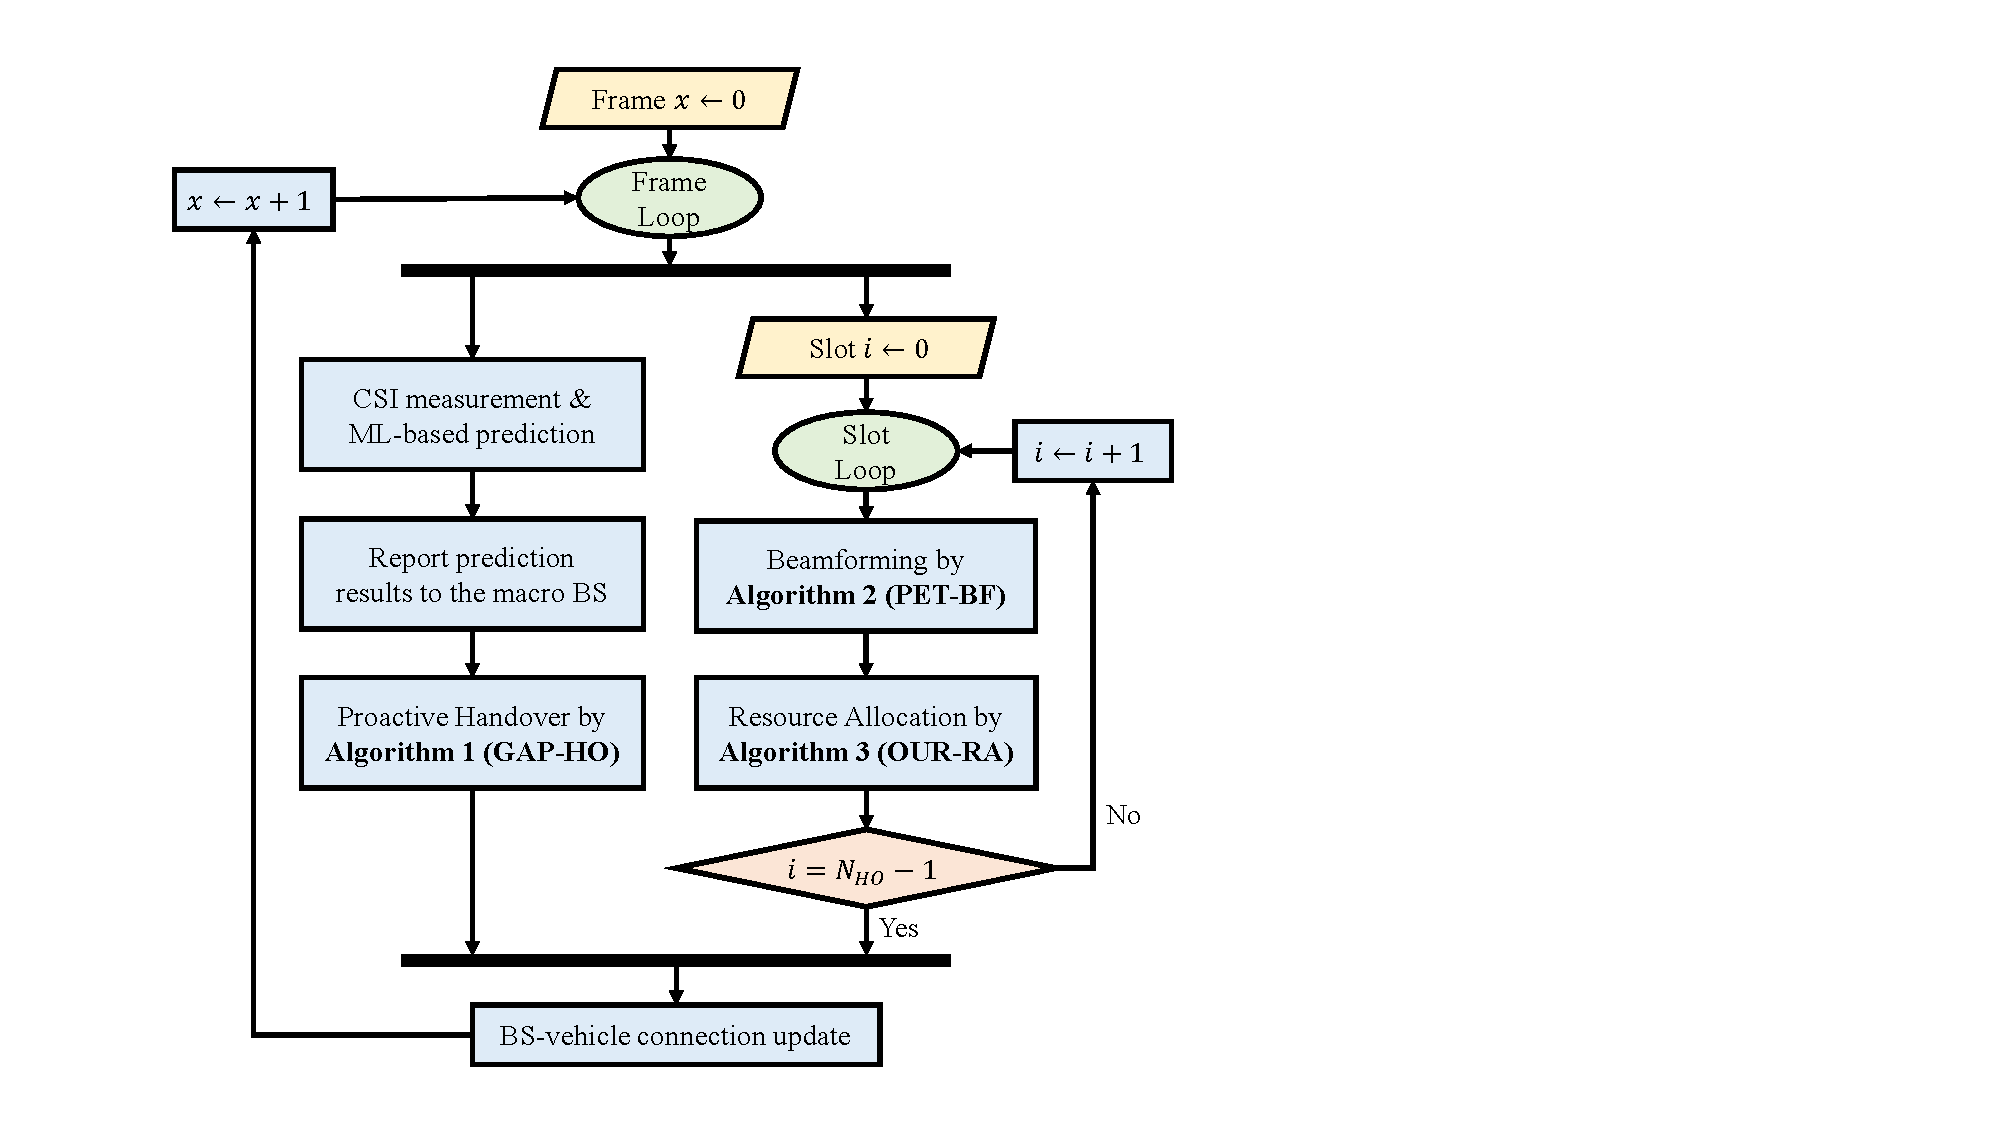
\includegraphics[width=0.5\textwidth, trim= 50 10 380 20,clip]{figures/flowchart.pdf}}
\caption{Flowchart of the MEET-COBRA framework.}
\label{fig:flow chart}
\end{figure}

% omit for 13 pages
\iffalse
    \begin{algorithm}[htbp]
        \caption{ML-Based Energy-Efficient Proactive Coordination of Handover, Beamforming and Resource Allocation (MEET-COBRA)}
        \label{alg:MEET-COBRA}
        \renewcommand{\algorithmicrequire}{\textbf{Input:}}
        \renewcommand{\algorithmicensure}{\textbf{Output:}}
        \begin{algorithmic}[1] % Control whether there are numbers
            \REQUIRE  % input contents
            $\mathcal{M}$, $N_0$, $N_{\textup{HO}}$, $M_{\rm T}$, $M_{\rm R}$, $M_{\rm P}$, $\zeta$, $\Delta t$, \currentdel{$\tau^{{\rm th}}$}\rev{$\tau_v^{\rm th}$}, $p_m$, $K_m$, $B_m$, $F_m$, $\lambda_v$, $\alpha$, $\beta$;
            
            \ENSURE % output contents
            $u_{m,v}^{[x]}$,
            ${\bm{w}_{\rm T}}_{m,v}^{[x]},{\bm{w}_{\rm R}}_{m,v}^{[x]}$,
            $k_{m,v}^{[x]}(i)$;
    
            \STATE \textbf{Initialization:}  $\mathcal{V}^{[-1]} \leftarrow \emptyset$, $u_{m,v}^{[x]} \leftarrow 0$, $k_{m,v}^{[x]}(i) \leftarrow 0$;
            
            \FOR{$x = 0,1, 2, \ldots$}
                \STATE Newly arrived vehicles initially access to the macro BS and obtain the NN model: $u_{0,v}^{[x]} \leftarrow 1, \forall v \in \mathcal{V}^{[x]} \backslash \mathcal{V}^{[x-1]}$;
                
                \STATE Newly left vehicles hand over to another macro BS outside the region: $u_{m,v}^{[x]} \leftarrow 0, \forall m \in \mathcal{M}, \forall v \in \mathcal{V}^{[x-1]} \backslash \mathcal{V}^{[x]}$;
                
                \STATE Each vehicle measures ${\rm CSI}_v^{[x]}$, and executes ML-based prediction to obtain $\bigl\{\Tilde{\mathcal{P}}_{m,v}^{[x+1]}, \Tilde{G}_{m,v}^{[x+1]}, \Tilde{G}_{{\rm I},m,v}^{[x+1]}\bigr\}_{m=1}^M$;
    
                \STATE Each vehicle reports prediction results to the macro BS;
                
                \STATE The central PHO server executes Algorithm~\ref{alg:GAP-HO} to obtain $u_{m,v}^{[x+1]}$ and initiates the PHO process for the next frame;
                
                \FOR {$i=0,1, 2, \ldots,N_{\textup{HO}}-1$}
                    
                    \STATE Execute Algorithm~\ref{alg:predictive BF} to obtain BF vectors ${\bm{w}_{\rm T}}_{m,v}^{[x]}(i)$ and ${\bm{w}_{\rm R}}_{m,v}^{[x]}(i), \forall m \in \mathcal{M}\backslash\{0\}, \forall v\in \mathcal{V}^{[x]}_m$;
    
                    \STATE Execute Algorithm~\ref{alg:OTR-RA} to obtain RB allocations $k_{m,v}^{[x]}(i), \forall m \in \mathcal{M}, \forall v\in \mathcal{V}^{[x]}_m$;
                                
                    \STATE Each BS conducts downlink transmission;
                \ENDFOR
                \STATE Finish PHO process to update data-plane connections;
            \ENDFOR
            \STATE \textbf{return} 
        \end{algorithmic}
    \end{algorithm}
\fi

The proposed MEET-COBRA framework integrates the above modules into a unified two-timescale design, as illustrated in Fig.~\ref{fig:flow chart}.
% omit for 13 pages
% and summarized in Alg.~\ref{alg:MEET-COBRA}. 
Frame-level PHO decisions are computed centrally at the macro BS, while slot-level BF and RA are executed locally at each BS. 

At the beginning of frame-$x$, each vehicle performs local NN inference based on its historical CSI measurements to generate next-frame predictions $\{\Tilde{\mathcal{P}}_{m,v}^{[x+1]}, \Tilde{G}_{m,v}^{[x+1]}, \Tilde{G}_{{\rm I},m,v}^{[x+1]}\}$\currentdel{, which are reported to the macro BS through the control-plane uplink.}\rev{. Each vehicle reports only the top-$M_{\rm P}$ beam-pair indices in descending order of predicted probability and the two gain predictions for each micro BS to the macro BS through the control-plane uplink.} Using these predictions, the macro BS executes GAP-HO to compute the PHO decisions $u_{m,v}^{[x+1]}$ for the next frame. \rev{The macro BS also forwards the interfering-link gain predictions and estimated RB usages required by OTR-RA to the corresponding serving BSs before frame-$(x+1)$ begins.}

Within each slot-$i$ of frame-$x$, each micro BS-$m$ first applies PET-BF to probe the predicted top-$M_{\rm P}$ beam-pairs with early termination, thereby obtaining BF vectors $\{{\bm{w}_{\rm T}}_{m,v}^{[x]}(i), {\bm{w}_{\rm R}}_{m,v}^{[x]}(i)\}$ and instantaneous link gains $g_{m,v}^{[x]}(i)$ with limited beam-training overhead $\eta_{m,v}^{[x]}(i)$. 
After that, each BS applies OTR-RA to prioritize users by their RB efficiency $\Gamma_{m,v}^{[x]}(i)$ and perform queue-aware tiered-rounding to obtain integer RB allocations $k_{m,v}^{[x]}(i)$ under the RB-capacity constraints.

% \noindent\textbf{Key Insight:}
Remarkably, ML-based prediction serves as the coupling mechanism that aligns the modeling assumptions across HO, BF, and RA. The gain predictions enable GAP-HO to estimate the next-frame RB demands of each BS-vehicle pair and to solve \textbf{P2} based on a forward-looking characterization of the network state, while the beam-pair predictions guide PET-BF to realize high-quality beam alignment under reduced beam-training overhead. This improves the consistency between the link gains assumed in the RB-demand estimation of GAP-HO and the link gains realized during data transmission. Based on these realized link gains, OTR-RA further exploits opportunistic scheduling and queue-aware tiered rounding to enhance latency performance and reduce RB wastage, thereby narrowing the gap between the RB demands predicted by GAP-HO and the realized long-term RB usage. Consequently, MEET-COBRA provides a low-complexity online solution that effectively addresses the original problem \textbf{P1}.


\rev{Prediction errors can also affect this coordination. With other inputs fixed, overestimating the desired-link gain or underestimating the interfering-link gains lowers the estimated RB demand in~\eqref{eq:RB_demand_hat}, whereas errors in the opposite direction raise it. These changes affect the estimated power costs and RB requirements in GAP-HO, and can change BS--vehicle associations. In PET-BF, beam prediction errors affect the candidate beam-pair list and the search order, while desired-link gain errors affect the early-termination threshold. Both types of error can affect the gain of the selected beam pair and the beam-search overhead. OTR-RA uses measured desired-link gains, but errors in predicted interfering-link gains and estimated BS RB usages can affect RB-efficiency estimates, user ordering, and RB allocations. These effects can change transmit power and received rates, thereby influencing queue evolution and the violation probability $U$.}

\section{Simulation Results}

In this section, we evaluate the performance of the proposed MEET-COBRA framework using a simulation platform built on the SUMO~\cite{behrisch2011sumo} and the Sionna RT~\cite{sionnaRT} simulators.
We first describe the simulation setup and parameter configuration, and then present numerical results that compare MEET-COBRA with several baseline schemes in terms of power consumption and latency performance.

\subsection{Simulation Setup}

\begin{table*}[htbp]
    \centering
    \caption{Simulation Parameters}
    \label{tab:sim-params}
    \setlength{\tabcolsep}{4pt}
    \begin{tabular*}{\textwidth}{@{\extracolsep{\fill}}l c | l c c}
        \hline
        \multicolumn{2}{c|}{\textbf{Global simulation parameters}}
        & \multicolumn{3}{c}{\textbf{Macro- and micro-BS parameters}} \\
        \hline
        \textbf{Parameter} & \textbf{Value}
        & \textbf{Parameter} & \textbf{Macro BS} & \textbf{Micro BS} \\
        \hline
        Slot duration $\Delta t$ & $1$~ms
        & Carrier frequency $f_m$ & $2.8$~GHz & $28$~GHz \\

        PHO frame length $N_{\rm HO}$ & $100$ slots
        & Number of RBs $K_m$ & $133$ & $66$ \\

        Pilots per frame $N_{\rm P}$ & $8$
        & RB bandwidth $B_m$ & $0.36$~MHz & $1.44$~MHz \\

        Rician factor $K_{\rm R}$ & $3$
        & Per-RB transmit power $p_m$ & $1$~W & $0.2$~W \\

        Beam-search overhead $\eta$ & $2/112$
        & Noise figure $F_m$ & $5$~dB & $10$~dB \\

        Latency threshold \currentdel{$\tau_{\rm th}$}\rev{$\tau_v^{\rm th}$} & $20$~ms
        & Channel simulation &
        3GPP TR~38.901 UMa & Ray-tracing by Sionna RT~\cite{sionnaRT} \\

        \rev{HO interruption duration $\tau_{\rm HO}$} & \rev{$10$~ms}
        & Antenna number (Tx\&Rx) & 1\&1 & 32\&8 \\

        \rev{Number of GAP-HO iterations $N_{\rm iter}$} & \rev{$2$}
        & \rev{Number of BSs} & \rev{$1$} & \rev{$4$}\\

        \rev{RB capacity relaxation factor $\zeta$} & \rev{$1.1$}
        & \rev{Beamforming codebooks} & \rev{Not applicable} & \rev{DFT} \\

        Noise power spectral density $N_0$ & $-174$~dBm/Hz
        & \rev{Number of candidate beam pairs $M_{\rm P}$} & \rev{Not applicable} & \rev{$5$} \\

        \rev{System simulation duration per run} & \rev{$30$~s}
        & \rev{PET-BF gain margin $G_{\rm th}$} & \rev{Not applicable} & \rev{$5$~dB} \\
        \hline
    \end{tabular*}
\end{table*}

\begin{figure}
\centerline{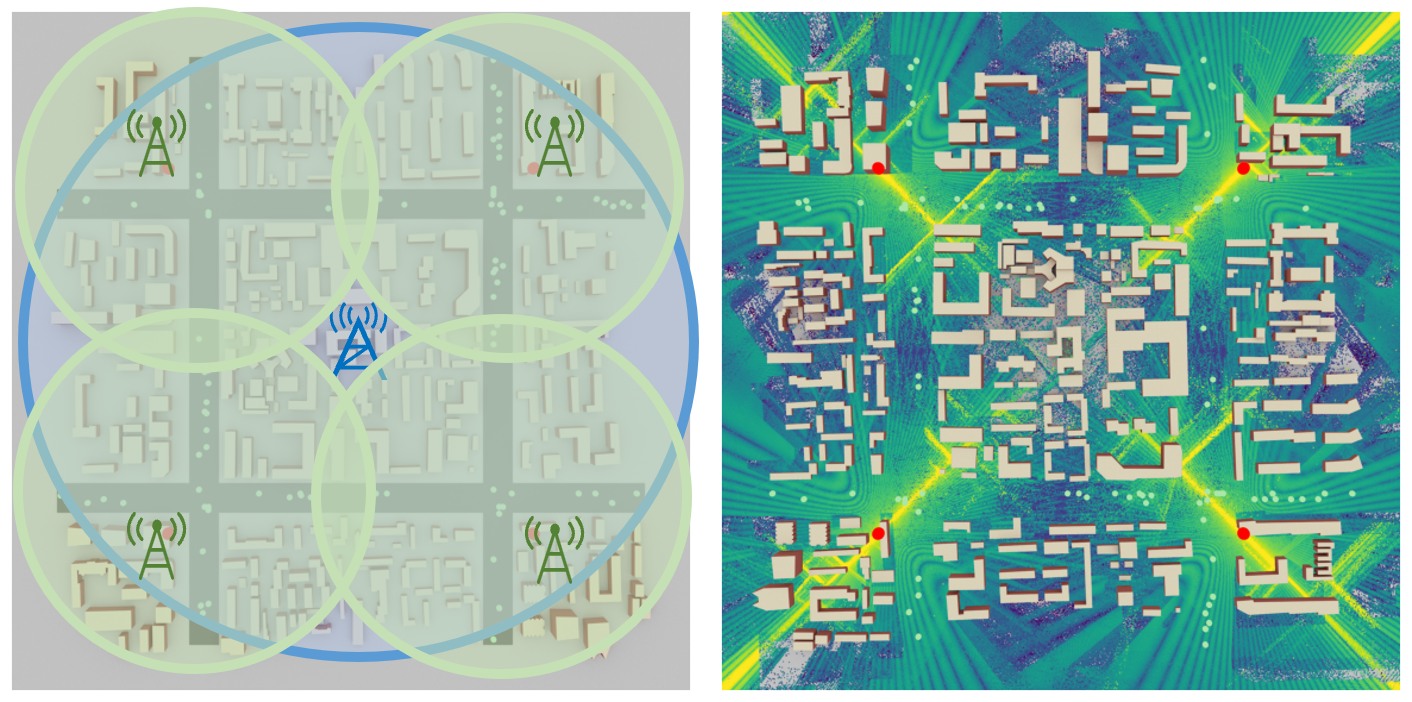
\includegraphics[width=0.5\textwidth, trim= 0 0 0 0,clip]{figures/Sionna Simulation.png}}
\caption{Simulation scenario of the considered two-tier HetNet. Left: road layout, buildings, and \currentdel{locations/coverage regions}\rev{locations and coverage regions} of the macro BS (blue) and four micro BSs (green). Right: example Sionna RT ray-tracing–based received-power map at $28$~GHz with vertically polarized antennas and micro-BS ULAs oriented toward the area center.}
\label{fig:simulation scenario}
\end{figure}


We consider a $1000~\text{m} \times 1000~\text{m}$ urban HetNet scenario shown in Fig. \ref{fig:simulation scenario}, where one macro BS is deployed at the center $(0,0)$ and four micro BSs are located at $(\pm 300,\pm 300)$~m. The road topology consists of four intersections centered at $(\pm 250,\pm 250)$~m, and each road segment is bidirectional with three lanes per direction. Each micro BS employs a ULA oriented toward the scenario center. All antennas are vertically polarized. \currentdel{Realistic vehicular mobility trajectories are first generated using the SUMO traffic simulator; based on these trajectories, Sionna RT simulator is used to obtain the time-varying MIMO channel matrices between each vehicle and each micro BS, while the large-scale channel gains between vehicles and the macro BS are generated according to the 3GPP TR~38.901 urban macro model~\mbox{\cite{3GPP-TR-38.901}}. Unless otherwise stated, the main simulation parameters are summarized in Table~\mbox{\ref{tab:sim-params}}.}\rev{SUMO generates the vehicle trajectories, which are used by Sionna RT to obtain the time-varying MIMO channel matrices between vehicles and micro BSs. The large-scale channel gains between vehicles and the macro BS are generated using the 3GPP TR~38.901 urban macro model~\cite{3GPP-TR-38.901}.}

\begin{figure}[t]
    \centering
    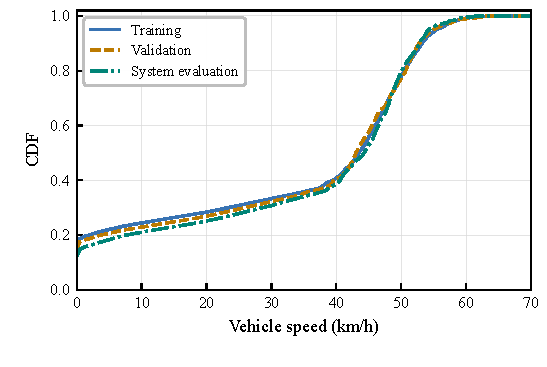
\includegraphics[width=\columnwidth]{figures/vehicle_speed_cdf_revision1.pdf}
    \caption{\rev{Vehicle-speed CDFs over vehicle-frame samples from the training, validation, and system evaluation datasets.}}
    \label{fig:vehicle-speed-cdf}
\end{figure}

\rev{Fig.~\ref{fig:vehicle-speed-cdf} shows the cumulative distribution functions (CDFs) of vehicle speed in the training, validation, and system evaluation datasets. The respective mean speeds are $33.56$, $33.95$, and $34.78$~km/h. Samples with zero speed account for $14.97\%$, $14.64\%$, and $12.07\%$ of the corresponding vehicle-frame observations. Vehicle speeds in the system evaluation dataset range from 0 to 61.53 km/h.}

\rev{For the system-level performance comparisons in Section~V-D, we vary the traffic arrival rate $\lambda_v=\lambda$ over $\{1,3,\ldots,35\}$~Mbps and set $\tau_v^{\rm th}=20$~ms for all vehicles.}
\rev{For all schemes, receive rates are evaluated using actual RB overlaps and the selected transmit and receive beams.}
\rev{We set $N_{\rm iter}=2$ to balance performance and computational cost, and $\zeta=1.1$ for 10\% increments in the RB capacity bounds when the continuous relaxation of \textbf{P2} is infeasible. We use $M_{\rm P}=5$ and $G_{\rm th}=5$~dB to balance coverage of the optimal beam pair against beam search overhead, which occupies at most $\eta M_{\rm P}=8.93\%$ of each slot.}
\rev{Unless otherwise stated, the simulations use the parameter values listed in Table~\ref{tab:sim-params}.}

\subsection{Performance of ML-Based Prediction}

We evaluate the NN models in Section~\ref{subsection: ML pred} for beam-pair and gain prediction.
% Fig. 4 now uses the retrained beam-average interfering-gain predictor:
% experiment/results/revision_directional_20260922/fig4_summary.json.
% The beam and desired-gain histories remain unchanged.
We set $N_{\rm C}=128$ for the LSTM unit and the vector ResBlock, with $N_{\rm H}=4$ vector ResBlocks per output head.
\currentdel{The dataset is built from $6000$ frames of Sionna RT–generated channel traces, with about $136$ active vehicles per frame on average. To avoid information leakage, the data samples used for training and validation are taken from non-overlapping time intervals. Each sample consists of the historical CSI of a vehicle over $1\text{-}10$ consecutive frames, together with labels of the optimal beam-pair indices and the corresponding desired-link and interference-link gains for the next frame. The samples are randomly split into training (70\%) and validation (30\%) sets.}\rev{The dataset is built from Sionna RT–generated channel traces spanning $6000$ frames and contains $646{,}747$ labeled samples from $706$ vehicles. Each sample consists of the current-frame CSI of a vehicle, together with labels of the optimal beam-pair indices and the desired-link and \rev{beam-averaged }interfering-link gains for the next frame. The dataset is randomly partitioned at the vehicle level, with 70\% of the vehicles in the training set and the remaining 30\% in the validation set.
%This vehicle-level split is fixed for both training stages.
}

\currentdel{All models are trained offline for $100$ epochs using the AdamW~\mbox{\cite{adamw}} optimizer with a learning rate of $10^{-3}$ and a weight decay of $10^{-4}$.}\rev{All models are trained offline in two stages of $100$ epochs each, using AdamW~\cite{adamw} with a weight decay of $10^{-4}$. In the first stage, the models are randomly initialized and trained using the input windows of one to ten consecutive CSI frames at a learning rate of $10^{-3}$. 
In the second stage, the models are initialized from the best first-stage checkpoints for stateful fine-tuning. This stage uses an initial learning rate of $10^{-4}$ and truncated backpropagation through time~\cite{williams1990tbptt} with a truncation length of ten frames.
Recurrent states $\bm{h}_v$ and $\bm{c}_v$ are carried across frames and reset only at the start of a new trajectory. 
Both training and validation use finite input windows in the first stage and process samples in time order along each vehicle trajectory in the second. In both stages, the beam checkpoint is selected by the highest top-1 validation accuracy and each gain checkpoint by the lowest validation MAE. The selected second-stage checkpoints are used in all subsequent evaluations.}
% Revision TODO: Regenerate Figs. 5--8 with stateful inference using the selected
% model bundle in experiment/results/revision_directional_20260922/selected_models.


\begin{figure}[htbp]
    \centering
    \subfloat[Beam prediction model.]{%
        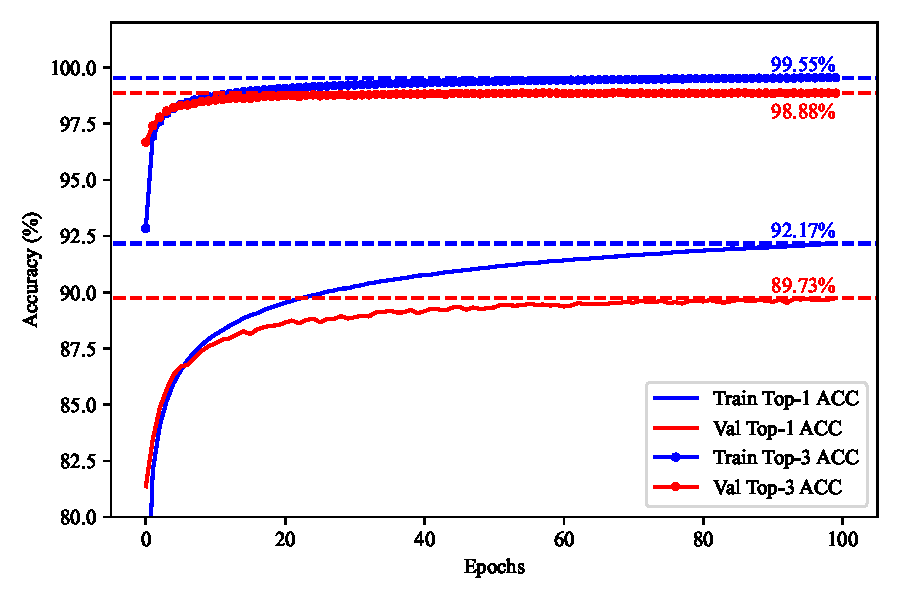
\includegraphics[width=0.95\columnwidth]{figures/NN_training_curves(a).pdf}%
        \label{fig:nn-train-a}}
    \vfill
    \subfloat[Gain prediction models.]{%
        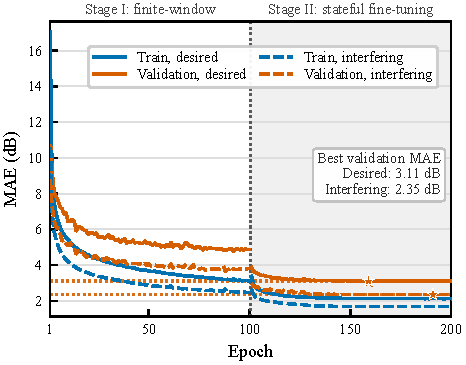
\includegraphics[width=0.95\columnwidth]{figures/NN_training_curves(b).pdf}%
        \label{fig:nn-train-b}}
    \caption{Training and validation performance of the proposed NN models:
    (a) beam prediction model (\currentdel{top-1/top-3 accuracy}\rev{top-1 and top-3 accuracies});
    (b) optimal desired-link and \currentdel{interference-link}\rev{interfering-link} gain prediction models (MAE). \rev{The vertical dotted line separates finite-window training (epochs 1--100) and stateful fine-tuning (epochs 101--200). Stars mark the best validation value of each metric.}}
    \label{fig:nn-train}
\end{figure}

Fig.~\ref{fig:nn-train} illustrates the training and validation performance of the beam and gain prediction models.
\currentdel{For the beam prediction model, the top-1 accuracy on the validation set converges to about $89.7\%$, while the top-3 accuracy reaches approximately $98.9\%$, with a small gap between the training and validation curves, indicating good generalization.}\rev{Stateful fine-tuning increases the best top-1 validation accuracy of beam prediction from $86.68\%$ to $89.16\%$ and achieves a best top-3 validation accuracy of $98.65\%$.}
\currentdel{Besides, we also evaluate the top-$M_{\rm P}$ reliability of the beam prediction, which exceeds $99\%$ for $M_{\rm P} \geq 4$ and $99.9\%$ for $M_{\rm P} \geq 18$, implying that the optimal beam-pair is almost always contained in a short candidate list.}\rev{For the selected beam checkpoint, the validation top-$M_{\rm P}$ accuracy exceeds $99\%$ for $M_{\rm P} \geq 4$ and $99.9\%$ for $M_{\rm P} \geq 17$, indicating that a short candidate list contains the optimal beam pair with high probability.}
\currentdel{For the gain prediction models, the validation mean absolute error (MAE) stabilizes around $4.1$~dB for the optimal desired-link gain and $3.2$~dB for the interference-link gain, and the training/validation curves nearly overlap.}\rev{Stateful fine-tuning also reduces the best validation MAEs of desired-link and \rev{beam-averaged }interfering-link gain prediction from $4.79$ and \rev{$3.85$}~dB to $3.11$ and \rev{$2.51$}~dB, respectively.}
\currentdel{These results confirm that the NN models provide sufficiently accurate beam and gain predictions to support MEET-COBRA.}\rev{These results show improved beam and gain prediction after stateful fine-tuning.} \rev{We further assess the selected models across four speed groups of $[0,1)$, $[1,20)$, $[20,40)$, and $\geq40$~km/h on the system evaluation dataset.
From the lowest to the highest speed group, the desired-link gain MAEs are $1.13$, $2.31$, $3.15$, and $3.73$~dB, and the corresponding interfering-link gain MAEs are $1.19$, $1.79$, $2.32$, and $3.07$~dB. Top-5 beam prediction accuracy exceeds $99\%$ in all four groups.}

\begin{table}[tbp]
    \centering
    \color{revisioncolor}
    \caption{NN Parameter Counts and Inference FLOPs}
    \label{tab:nn-overhead}
    \small
    \begin{tabular}{lrc}
        \toprule
        Predictor & Parameters & {Matrix FLOPs ($10^6$)} \\
        \midrule
        Beam-pair & 1,060,864 & 2.10 \\
        Desired-link gain & 533,524 & 1.05 \\
        Interfering-link gain & 533,524 & 1.05 \\
        Total & 2,127,912 & 4.20 \\
        \bottomrule
    \end{tabular}
    \par\smallskip
    \parbox{\columnwidth}{\footnotesize Matrix FLOPs count LSTM and linear-layer matrix operations, with two FLOPs per multiply--accumulate.}
\end{table}

\rev{Table~\ref{tab:nn-overhead} summarizes the NN parameter counts and matrix FLOPs for single-vehicle stateful inference using the current-frame CSI and recurrent states. The three models require 8.51~MB of 32-bit floating-point (FP32) parameter storage. With FP32 inference on an AMD EPYC 
7742 CPU using one thread, their combined inference latency has a median of \rev{5.38} ms and a 95th percentile of \rev{5.72} ms. With $M=4$, $M_{\rm P}=5$, and $M_{\rm T}M_{\rm R}=256$, each vehicle reports, for each micro-BS link, $M_{\rm P}$ beam-pair indices in descending order of predicted probability, using 8 bits per index, together with one FP32 desired-link gain and one FP32 interfering-link gain. The \rev{reporting overhead} is $M(8M_{\rm P}+2\times32)=416$ bits per vehicle per frame (4.16~kbps). At the same reporting interval and 32-bit precision per real CSI component, this reduces \rev{reporting overhead} by factors of 157.5 and 9.85 relative to full MIMO-CSI reporting and centralized inference using current-frame superposed-pilot observations, respectively.}

% TODO 暂时不讲，视篇幅情况看是否加入
%To examine the impact of model input design, Fig.~\ref{fig:nn-design} depicts the validation performance versus the number of pilots $N_{\rm P}$ and the CSI input length $N_{\rm L}$. Increasing $N_{\rm P}$ from $2$ to $8$ significantly improves beam prediction accuracy and reduces gain-prediction MAE, whereas further enlarging $N_{\rm P}$ yields only marginal gains, demonstrating a clear diminishing-returns effect. A similar trend is observed when increasing $N_{\rm L}$: performance improves rapidly for short histories and then saturates when $N_{\rm L} \gtrsim 10$. Unless otherwise stated, we therefore adopt $N_{\rm P}=8$ and $N_{\rm L}=10$ in the subsequent simulations as a good tradeoff between prediction accuracy and pilot/feedback overhead.


\subsection{Benchmark Schemes}
\label{subsec:benchmarks}

To assess the performance of MEET-COBRA, we compare it with the following benchmark schemes:

% omit for 13 pages

%\textbf{1) Oracle-MC:} This scheme corresponds to MEET-COBRA with perfect CSI and beam knowledge: all NN predictions are replaced by their true values obtained from the simulator. It reflects the performance loss caused by the NN prediction errors in MEET-COBRA.
\textbf{1) Oracle-MC:} MEET-COBRA with perfect beam and gain knowledge, where all ML predictions are replaced by their ground-truth values from the simulator. It quantifies the performance loss due to prediction errors.

%\textbf{2) Oracle-CR-LB:} Assuming perfect CSI and beam knowledge, this benchmark solves the continuous relaxation of \textbf{P2} by relaxing the binary association variables $u_{m,v}^{[x+1]} \in \{0,1\}$ to continuous variables in $[0,1]$. The optimal objective value of the relaxed problem provides a theoretical lower bound on the minimum system transmit power required to satisfy the latency constraint. If the relaxed problem is infeasible, the system transmit power is set to the maximum value corresponding to the full RB utilization of all BSs. As the relaxed solution is generally not implementable, Oracle-CR-LB is used only as a power lower bound and no meaningful latency constraint violation probability is reported for this scheme.
\currentdel{\textbf{2) Oracle-CR-LB:} A non-implementable power lower bound obtained by solving the continuous relaxation of \textbf{P2} (i.e., relaxing $u^{[x+1]}_{m,v}\in\{0,1\}$ to $[0,1]$) with perfect beam and gain knowledge. If the relaxed problem is infeasible, the full-load power ceiling is reported. No latency metric is reported for this unrealistic scheme.}

%\textbf{3) Reactive-OBRA:} This scheme corresponds to a reactive HetNet baseline without ML-based prediction or proactive coordination among HO, BF, and RA. In this scheme, HO follows a load-aware and channel-quality-driven rule in HetNets~\cite{Alexandris2016LoadAwareHO}: each vehicle associates with the micro BS offering the largest received signal strength (RSS), and falls back to the macro BS when that micro BS is overloaded. BF follows a low-complexity, random opportunistic search baseline inspired by~\cite{Aykin2020}: whenever a vehicle hands over to a new micro BS, the BS randomly probes $M_{\rm P}$ beam-pairs and selects the one with the highest measured gain; in subsequent slots, it keeps probing random candidates and updates the serving beam-pair only if a better one is found. For RA, each BS assumes all interfering micro BSs operate at full load when estimating RB efficiency, and obtains integer RB allocations via stochastic rounding.
\textbf{\currentdel{3}\rev{2}) Reactive-OBRA:} A reactive HetNet baseline without ML prediction or proactive coordination. \currentdel{HO is received signal strength (RSS)-based. When the serving BS is overloaded, users are offloaded to the nearest available BS~\mbox{\cite{Alexandris2016LoadAwareHO}}.}\rev{Using current channel gains, it assigns vehicles sequentially to the BS with the lowest estimated transmit power cost among those with sufficient remaining RB capacity, falling back to the macro BS if none is available.} BF uses a random opportunistic search inspired by~\cite{Aykin2020}: after HO it probes $M_{\rm P}$ beam-pairs and keeps randomly probing thereafter, updating the serving beam only when a better one is found. RA estimates RB efficiency assuming full-load interfering micro BSs and applies stochastic rounding for integer RB allocation.


%\textbf{4) Ablation variants of MEET-COBRA:} We also consider three ablation schemes, denoted {w/o GAP-HO}, {w/o PET-BF}, and {w/o OTR-RA}. In each scheme, one of the HO, BF, or RA modules in MEET-COBRA is replaced by its counterpart in Reactive-OBRA, while the other two modules remain unchanged. These variants isolate the individual contributions of GAP-HO, PET-BF, and OTR-RA to the overall performance of MEET-COBRA.
\textbf{\currentdel{4}\rev{3}) Ablations:} \emph{w/o GAP-HO}, \emph{w/o PET-BF}, and \emph{w/o OTR-RA}, where the corresponding module in MEET-COBRA is replaced by its Reactive-OBRA counterpart, while keeping the other two modules unchanged.

\rev{\textbf{4) O-MAPPO-adapted:} This baseline adapts the O-MAPPO framework in~\cite{wang2024joint}, which combines reinforcement learning with target BS optimization. A shared actor trained by multi-agent proximal policy optimization evaluates whether each vehicle should trigger HO after every 10~m of travel. For vehicles with active HO triggers, a mixed-integer optimizer selects target BSs using estimated RB demands, BS loads, and transmit power costs, with penalties for aggregate demands exceeding BS capacities. The actor and optimizer use the same predicted desired-link and interfering-link gains as MEET-COBRA. Association changes take effect in the next frame. Upon HO to a micro BS, hierarchical beam search starts after the HO interruption. It first probes all combinations of eight transmit and two receive sectors, then all combinations of four transmit and four receive DFT beams within the selected sectors, requiring 32 probes in total. In subsequent slots, local beam tracking probes the current beam pair and four adjacent pairs differing in only one beam index, and then \rev{retains} the pair with the highest measured gain. Each BS applies OTR-RA in every slot.}

\rev{\textbf{5) MTS-GS-HBF-adapted:} This baseline adapts the multi-timescale association and hybrid BF framework in~\cite{heydarian2025multitimescale}. Gale--Shapley matching updates BS--vehicle associations every five frames using the same predicted channel gains as MEET-COBRA. Matching preferences account for estimated rates, BS loads, queue backlogs, and energy and HO costs, while association decisions consider estimated RB demands and BS capacities. We replace the original hybrid BF with the hierarchical beam search and local tracking used in O-MAPPO-adapted. Unlike O-MAPPO-adapted, hierarchical beam search is repeated in the first available slot of every frame, after the HO interruption when applicable, followed by local beam tracking in the remaining slots. Each BS applies OTR-RA in every slot.}

\subsection{Performance Comparison}

% Submitted text is retained only as deletion markup, not as an intermediate draft.
\ifshowdeletions
\currentdel{This subsection compares MEET-COBRA with all benchmark schemes under the same mobility traces and traffic statistics. For each simulation setting, we run the system for a $30$~s horizon (i.e., $300$ frames) and report metrics time-averaged over this horizon.}

\currentdel{Fig.~\mbox{\ref{fig:power_comparison_curves}} and Fig.~\mbox{\ref{fig:violation_prob_comparison_curves}} compares the average system transmit power $\bar{P}$ and the latency constraint violation probability $U$ under different data arrival rates $\lambda$ (with $M_{\rm P}=5$ and other parameters in Table~\mbox{\ref{tab:sim-params}}).
To facilitate interpretation, we partition the network load into three regimes using $\lambda=20$ and $30$~Mbps as coarse thresholds, and summarize the key observations as follows:}

\currentdel{\emph{Light-load regime ($\lambda<20$~Mbps):}
    $\bar{P}$ increases approximately linearly with $\lambda$ and latency violations are negligible.
    For instance, at $\lambda=19$~Mbps, MEET-COBRA achieves $\bar{P}=44.38$~W with $U=0.34\%$, approaching Oracle-MC ($40.86$~W), which indicates only a marginal performance loss due to NN prediction errors.
    Moreover, Oracle-MC nearly coincides with Oracle-CR-LB in this regime, suggesting that, when perfect CSI/beam knowledge eliminates the prediction errors, the resulting performance is close to the theoretical power lower bound; this shows the near-optimality of the proposed MEET-COBRA framework under light loads.}

\currentdel{\emph{Medium-load regime ($20\le\lambda<30$~Mbps):}
    RB-capacity constraints become active for some micro BSs and load imbalance emerges. GAP-HO performs global BS-vehicle association optimization, thereby balancing per-BS RB usage and maintaining low $\bar{P}$ and $U$. For example, at $\lambda=27$~Mbps, MEET-COBRA achieves $(\bar{P},U)=(125.82~\text{W},0.68\%)$, whereas Reactive-OBRA already reaches the RB-capacity-imposed power ceiling (about $185.4$~W) and suffers a much higher $U=29.47\%$.
    Moreover, Fig.~\mbox{\ref{fig:violation_prob_comparison_curves}} exhibits a non-monotonic behavior of $U$ in this regime, where several curves (especially MEET-COBRA, w/o OTR-RA, and w/o PET-BF) temporarily flatten or slightly decrease before rising again. This mainly stems from GAP-HO offloading vehicles from some RB-limited micro BSs to the macro BS, thereby reducing network congestion and inter-cell interference.}

\currentdel{\emph{Heavy-load regime ($\lambda\ge 30$~Mbps):}
    The network approaches full RB utilization and $\bar{P}$ saturates around the power ceiling, while $U$ increases rapidly as the offered load exceeds the service capability.  At $\lambda=33$~Mbps, MEET-COBRA reaches $\bar{P}=185.4$~W with $U=26.08\%$, whereas Reactive-OBRA exhibits a substantially higher violation probability ($U=50.86\%$).}

\currentdel{The ablation results further reveal the distinct roles of GAP-HO, PET-BF, and OTR-RA across different network load states.
Under light loads, {w/o GAP-HO} almost overlaps with MEET-COBRA, suggesting that the near-optimal association is essentially to connect each vehicle to its best micro BS when the RB budgets of micro BSs are sufficient.
As the load increases, the performance loss of {w/o GAP-HO} grows rapidly and eventually becomes the most dominant among all ablation schemes, showing that global association optimization is crucial for load balancing once RB-capacity constraints become active.
Moreover, among the three ablation schemes, {w/o OTR-RA} causes the largest power increase for $\lambda<10$~Mbps, since conservative interference estimation (assuming full RB utilization for all interfering BSs) and stochastic rounding for RB allocation can lead to substantial resource wastage when the network is lightly loaded, whereas OTR-RA mitigates such wastage via more accurate interference estimation and queue-aware tiered-rounding.
Besides, {w/o PET-BF} degrades network performance across all load regimes, since both BF gain and beam-training overhead continuously impact link efficiency. PET-BF uses NN predictions with early termination to improve the BF gain while reducing training overhead, yielding consistent improvements irrespective of the traffic load.}

\currentdel{Fig.~\mbox{\ref{fig:latency_90th_99th_comparison_curves}} reports the 90th/99th-percentile user latency, denoted by $L_{90}$/$L_{99}$,
and Fig.~\mbox{\ref{fig:BS0_assoc_ratio_comparison_curves}} reports the macro-BS association ratio $\rho_{0}$ (in \%), i.e., the percentage of vehicles associated with BS-0.}

\currentdel{Under light loads, all schemes exhibit small $L_{90}$/$L_{99}$ and almost zero $\rho_{0}$ (e.g., MEET-COBRA achieves $\rho_{0}=0.03\%$ at $\lambda=19$~Mbps),
which is consistent with the observation that the RB budgets of each BS are sufficient and most vehicles can be served by favorable micro-BS links.}

\currentdel{As the load increases, the tail-latency behavior starts to differentiate and aligns well with the violation probability trends in Fig.~\mbox{\ref{fig:violation_prob_comparison_curves}}.
A salient metric is the first $\lambda$ at which $L_{99}$ exceeds the latency threshold $\tau_{\rm th}=20$~ms:
it occurs at $\lambda=29$~Mbps for MEET-COBRA,
whereas it happens much earlier for Reactive-OBRA ($\lambda=15$~Mbps), {w/o OTR-RA} ($\lambda=17$~Mbps), {w/o GAP-HO} ($\lambda=21$~Mbps), and {w/o PET-BF} ($\lambda=23$~Mbps).
This confirms that MEET-COBRA significantly delays the onset of tail latency degradation.}

\currentdel{Fig.~\mbox{\ref{fig:BS0_assoc_ratio_comparison_curves}} provides interpretable evidence on how each scheme redistributes load. At $\lambda=29$~Mbps, MEET-COBRA maintains a moderate macro-BS association ratio $\rho_{0}=16.50\%$ with only a mild tail-latency exceedance ($L_{99}=26.76$~ms, $U=1.14\%$). By contrast, Reactive-OBRA exhibits a much higher $\rho_{0}=35.18\%$ with a tail-latency collapse ($L_{99}=1.55\times 10^{4}$~ms, $U=37.46\%$), while w/o GAP-HO increases $\rho_{0}$ to $25.75\%$ and enlarges $L_{99}$ to $4.91\times 10^{3}$~ms with $U=18.54\%$.
Moreover, the mild non-monotonicity of $L_{99}$ in the medium-load regime in Fig.~\mbox{\ref{fig:latency_90th_99th_comparison_curves}} is similar to that of $U$ in Fig.~\mbox{\ref{fig:violation_prob_comparison_curves}}, which coincides with the initial rise of $\rho_0$ in Fig.~\mbox{\ref{fig:BS0_assoc_ratio_comparison_curves}}.
These results demonstrate that the globally optimized PHO of GAP-HO effectively balances network load under RB-capacity constraints, thereby delaying congestion build-up and mitigating extreme-tail latency.}

\currentdel{Finally, the joint use of Fig.~\mbox{\ref{fig:latency_90th_99th_comparison_curves}} and Fig.~\mbox{\ref{fig:BS0_assoc_ratio_comparison_curves}} helps disentangle the roles of PET-BF and OTR-RA {beyond} association decisions.
At $\lambda=29$~Mbps, {w/o PET-BF} and {w/o OTR-RA} have $\rho_{0}$ comparable to MEET-COBRA (18.88\% and 18.16\% versus 16.50\%), yet their tail latency is much worse ($L_{99}=5.71\times 10^{2}$~ms and $2.64\times 10^{2}$~ms, respectively).
Notably, {w/o PET-BF} also enlarges $L_{90}$ to 35.96~ms, indicating a latency performance degradation due to inefficient beam search without prediction-assisted candidate reduction and early termination,
whereas {w/o OTR-RA} keeps $L_{90}$ close to MEET-COBRA (2.14~ms versus 2.19~ms) but significantly enlarges $L_{99}$, suggesting that queue-aware tiered rounding mainly protects urgent users and mitigates extreme-tail violations.}
\fi

\rev{This subsection compares MEET-COBRA with the benchmark schemes in terms of transmit power and latency performance. At each data arrival rate, we run all schemes over the same $30$~s mobility trace with three random seeds. Each seed generates a different set of traffic arrivals and small-scale fading samples, which are shared by all schemes. Curves show the mean of the three runs, and shaded bands span their minimum and maximum values.}

\begin{figure}[t]
    \centering
    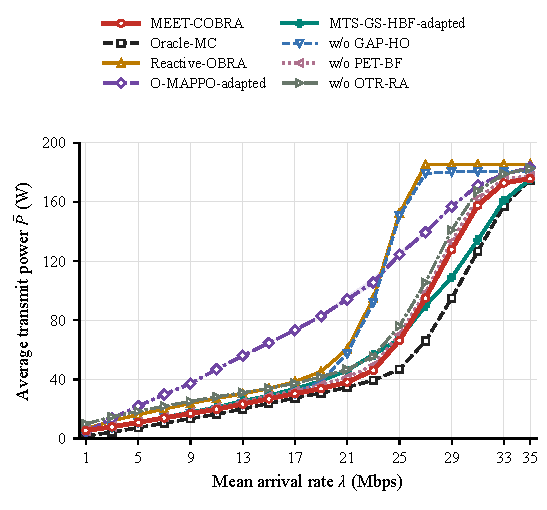
\includegraphics[width=\columnwidth]{figures/power_comparison_curves_revision1.pdf}
    \caption{Average system transmit power $\bar{P}$ versus the data arrival rate $\lambda$\currentdel{, where $\lambda$ is swept over $\{1,3,\ldots,35\}$~Mbps with $M_{\rm P}=5$ and other parameters given in Table~\mbox{\ref{tab:sim-params}}}.}
    \label{fig:power_comparison_curves}
\end{figure}

\begin{figure}[t]
    \centering
    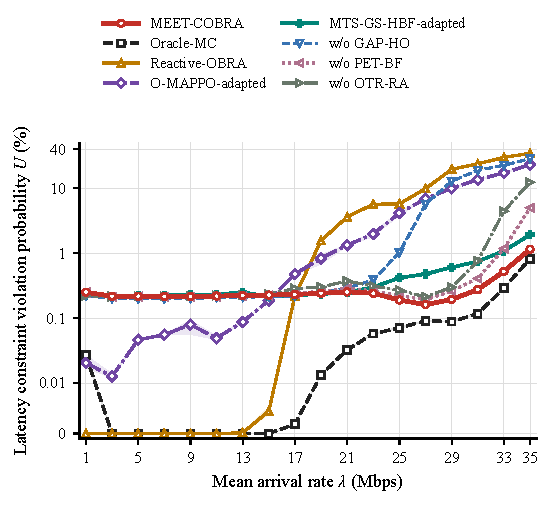
\includegraphics[width=\columnwidth]{figures/violation_prob_comparison_curves_revision1.pdf}
    \caption{Latency constraint violation probability $U$ versus the data arrival rate $\lambda$\currentdel{, where $\lambda$ is swept over $\{1,3,\ldots,35\}$~Mbps with $M_{\rm P}=5$ and other parameters given in Table~\mbox{\ref{tab:sim-params}}}. \rev{The vertical scale is linear below $0.01\%$ and logarithmic above it.}}
    \label{fig:violation_prob_comparison_curves}
\end{figure}

\rev{Figs.~\ref{fig:power_comparison_curves} and~\ref{fig:violation_prob_comparison_curves} compare the average system transmit power $\bar{P}$ and the latency constraint violation probability $U$, respectively, at different data arrival rates $\lambda$. Under light loads, the transmit power of MEET-COBRA increases approximately linearly with $\lambda$, as additional traffic can largely be accommodated by allocating more RBs without changing serving links. At $\lambda=19$~Mbps, MEET-COBRA uses $33.80$~W with $U=0.24\%$, compared with $30.71$~W and $0.013\%$ for Oracle-MC. This relatively small power gap suggests that prediction errors have a limited impact on transmit power when RB resources are sufficient. The power gap widens at $27$~Mbps, where the two schemes use $95.03$ and $66.00$~W, respectively. This larger power gap suggests that accurate RB-demand estimates become more important for coordinating PHO and RA when RB resources are limited.}

\rev{Compared with Reactive-OBRA, MEET-COBRA achieves much lower transmit power and fewer latency violations under heavy traffic. At $\lambda=27$~Mbps, Reactive-OBRA approaches the full-load power ceiling, using $185.39$~W with $U=9.84\%$, whereas MEET-COBRA uses $95.03$~W with $U=0.16\%$. These correspond to reductions of $48.7\%$ in transmit power and $98.4\%$ in violation probability. Further traffic increases mainly raise $U$ for Reactive-OBRA because its RB resources are already nearly fully utilized. MEET-COBRA maintains a low violation probability over a wider range of data arrival rates, although $U$ also increases as its RB resources approach full utilization. From $33$ to $35$~Mbps, its power increases only from $172.81$ to $175.80$~W, while $U$ rises from $0.52\%$ to $1.15\%$. Nevertheless, at $35$~Mbps, the violation probability of MEET-COBRA remains well below the $34.46\%$ observed for Reactive-OBRA.}

\rev{Compared with O-MAPPO-adapted, MEET-COBRA uses less power over $1$--$23$~Mbps and incurs fewer violations at every evaluated load. Over $25$--$33$~Mbps, O-MAPPO-adapted uses less power but incurs substantially more violations. At $29$~Mbps, O-MAPPO-adapted uses $107.40$~W with $U=4.18\%$, compared with $127.75$~W and $0.19\%$ for MEET-COBRA.}

\rev{Compared with MTS-GS-HBF-adapted, MEET-COBRA has lower mean power at every evaluated load and fewer violations at $\lambda\geq21$~Mbps. MTS-GS-HBF-adapted achieves slightly fewer violations at several lower loads. Its largest advantage in $U$ occurs at $1$~Mbps, with $0.23\%$ compared with $0.25\%$ for MEET-COBRA. At $29$~Mbps, MTS-GS-HBF-adapted uses $135.91$~W with $U=0.77\%$, both higher than the corresponding values of $127.75$~W and $0.19\%$ for MEET-COBRA. MTS-GS-HBF-adapted updates associations only every five frames, which can delay traffic redistribution when link conditions and queue backlogs change. Its periodic hierarchical beam search and local tracking also require more probes than PET-BF in MEET-COBRA. The additional probing leaves less time for data transmission, increasing the RB demand for a given link gain and amount of data to transmit.}

\begin{figure*}[t]
    \centering
    \subfloat[\rev{$L_{90}$ (90th percentile).}]{%
        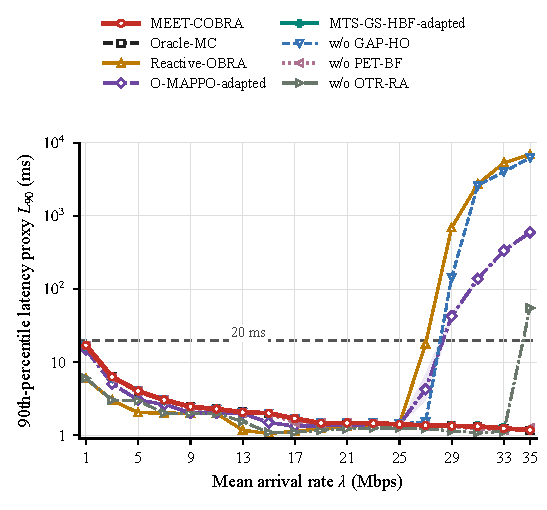
\includegraphics[width=0.49\textwidth]{figures/latency_90th_comparison_curves_revision1.pdf}%
        \label{fig:latency_90th_comparison_curves}}
    \hfill
    \subfloat[\rev{$L_{99}$ (99th percentile).}]{%
        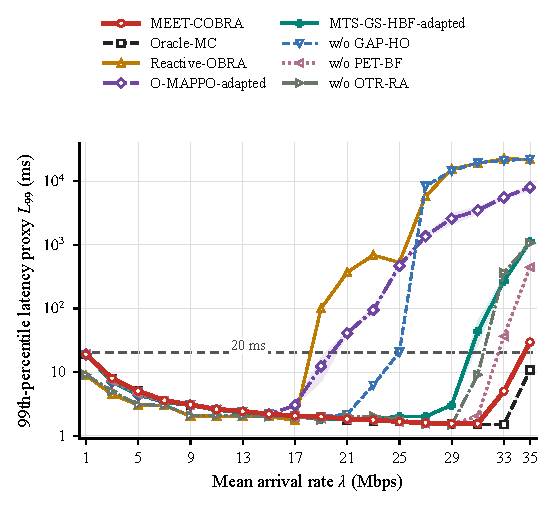
\includegraphics[width=0.49\textwidth]{figures/latency_99th_comparison_curves_revision1.pdf}%
        \label{fig:latency_99th_comparison_curves}}
    \caption{\currentdel{The 90th- and 99th-percentile user latency}\rev{The 90th and 99th percentiles of the queueing-delay proxy $\tau_v(n)$} versus the data arrival rate $\lambda$, where the horizontal dashed \currentdel{line denotes}\rev{lines denote} the latency threshold \currentdel{$\tau_{\rm th}=20$}\rev{$\tau_v^{\rm th}=20$}~ms.}
    \label{fig:latency_90th_99th_comparison_curves}
\end{figure*}

\begin{figure}[t]
    \centering
    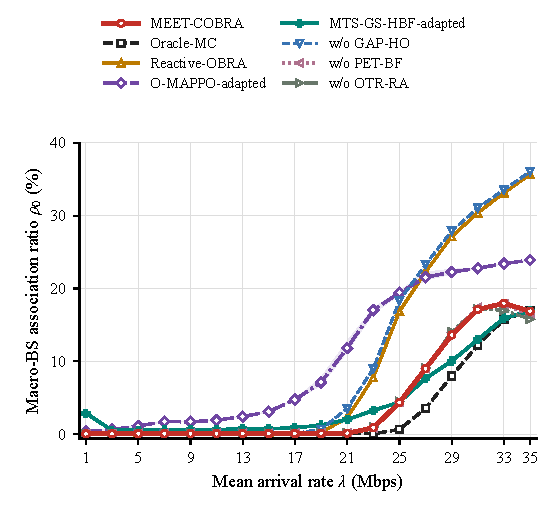
\includegraphics[width=\columnwidth]{figures/BS0_assoc_ratio_comparison_curves_revision1.pdf}
    \caption{Percentage of vehicles associated with the macro BS (BS-0) versus the data arrival rate $\lambda$.}
    \label{fig:BS0_assoc_ratio_comparison_curves}
\end{figure}

\rev{Fig.~\ref{fig:latency_90th_99th_comparison_curves} reports $L_{90}$ and $L_{99}$, the 90th and 99th percentiles of the queueing-delay proxy $\tau_v(n)$ over vehicle-slot samples within each run. As the arrival rate increases, $L_{99}$ can rise sharply while $L_{90}$ remains small. The mean $L_{99}$ first exceeds $20$~ms at $35$~Mbps for MEET-COBRA, compared with $19$~Mbps for Reactive-OBRA, $25$~Mbps for O-MAPPO-adapted and w/o GAP-HO, $31$~Mbps for MTS-GS-HBF-adapted, and $33$~Mbps for the other two ablations. Oracle-MC remains below this threshold throughout the evaluated range. At $33$~Mbps, MEET-COBRA and MTS-GS-HBF-adapted have similar $L_{90}$ values ($1.24$ and $1.19$~ms), but their $L_{99}$ values are $5.00$ and $267.54$~ms, respectively.} \rev{When evaluated separately for the speed groups $[0,1)$, $[1,20)$, $[20,40)$, and $\geq40$~km/h, MEET-COBRA maintains a mean $L_{99}$ below $20$~ms in every group at all evaluated arrival rates up to $33$~Mbps. At $35$~Mbps, the corresponding values are $1.49$, $11.19$, $28.37$, and $48.02$~ms in increasing speed-group order. These results indicate that MEET-COBRA maintains low latency across the observed speed groups over most evaluated loads, while larger delays arise in the higher-speed groups at the highest load.}

\rev{Fig.~\ref{fig:BS0_assoc_ratio_comparison_curves} reports the macro-BS association ratio $\rho_0$. MEET-COBRA serves almost all vehicles through micro BSs at light loads and offloads more traffic to the macro BS as the load increases. From $21$ to $27$~Mbps, $\rho_0$ rises from $0.14\%$ to $9.00\%$, while $U$ decreases from $0.25\%$ to $0.16\%$. This non-monotonic variation is consistent with GAP-HO redistributing traffic as micro-BS capacity constraints become limiting. At $29$~Mbps, MEET-COBRA maintains $\rho_0=13.61\%$ with $L_{99}=1.54$~ms, whereas Reactive-OBRA associates $27.13\%$ of vehicles with the macro BS and has $L_{99}>10^4$~ms. These results show the benefit of coordinating PHO, BF, and RA to serve traffic efficiently through the micro tier while balancing the traffic offloaded to the macro BS.}

\rev{However, a smaller macro-BS association ratio alone does not imply better load coordination. At $29$~Mbps, O-MAPPO-adapted has $\rho_0=7.74\%$, compared with $13.61\%$ for MEET-COBRA, but its $L_{99}$ reaches $364.76$~ms. At this load, the average micro-BS RB utilization is $97.2\%$ for O-MAPPO-adapted, compared with $79.8\%$ for MEET-COBRA. Retaining more traffic in the micro tier reduces the use of higher-power macro-BS RBs, but leaves little unused micro-BS capacity to clear accumulated queues. Moreover, O-MAPPO-adapted cannot reassign a vehicle without an active HO trigger, whereas GAP-HO reoptimizes BS--vehicle associations in every frame as resource demands change.}

\rev{The ablation results in Figs.~\ref{fig:power_comparison_curves}--\ref{fig:BS0_assoc_ratio_comparison_curves} further distinguish the contributions of the three modules of MEET-COBRA. Under light loads, w/o GAP-HO consumes almost the same power as MEET-COBRA, indicating limited additional power benefit from global PHO optimization when micro-BS RB resources are sufficient. As the load increases, its power and violation probability diverge from MEET-COBRA, reaching $179.27$~W and $5.67\%$ at $27$~Mbps. At this load, removing GAP-HO causes the largest increases in both metrics among the three ablations. Since w/o GAP-HO retains PET-BF and OTR-RA, this comparison highlights the importance of jointly coordinating BS--vehicle associations under capacity constraints, rather than assigning vehicles sequentially.}

\rev{Replacing PET-BF with random opportunistic beam search increases power throughout the evaluated range. PET-BF uses predicted beam-pair candidates to find a sufficiently strong beam pair and limits beam-search overhead through early termination. At $33$~Mbps, w/o PET-BF has $U=1.17\%$ and $L_{99}=36.41$~ms, compared with $0.52\%$ and $5.00$~ms for MEET-COBRA. These differences occur despite similar macro-BS association ratios ($17.87\%$ and $17.96\%$) and $L_{90}<1.3$~ms for both schemes, showing how efficient BF complements PHO in maintaining a small $L_{99}$.}

\rev{Removing OTR-RA causes the largest power increase among the ablations at light loads. Its replacement assumes full RB utilization at interfering BSs and uses stochastic rounding, whereas OTR-RA accounts for estimated RB usage and queue urgency. At $7$~Mbps, w/o OTR-RA uses $21.92$~W, compared with $13.95$~W for MEET-COBRA. Although the additional RB allocation can reduce latency under light loads, it leaves fewer RBs available as traffic increases. At $33$~Mbps, w/o OTR-RA has $L_{90}=1.13$~ms and $\rho_0=17.02\%$, close to the corresponding values of $1.24$~ms and $17.96\%$ for MEET-COBRA, but $U$ increases from $0.52\%$ to $4.40\%$ and $L_{99}$ from $5.00$ to $365.26$~ms. By rounding up RB allocations for urgent queues and rounding down those for nonurgent queues, OTR-RA reduces prolonged queue accumulation while limiting unnecessary RB use.}


\subsection{\rev{Impact of Gain-Prediction Errors}}
\label{subsection:gain-prediction-errors}

\begin{figure}[t]
    \centering
    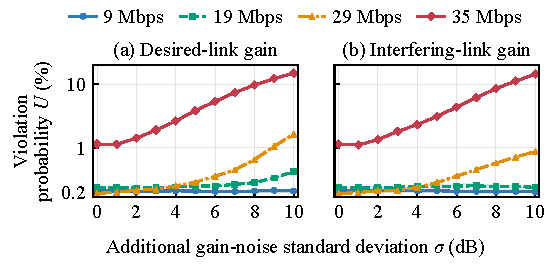
\includegraphics[width=\columnwidth]{figures/gain_error_sensitivity_revision1.pdf}
    \caption{\rev{Sensitivity of the latency constraint violation probability $U$ to gain-prediction errors.}}
    \label{fig:gain-error-sensitivity}
\end{figure}

\begin{figure}[t]
    \centering
    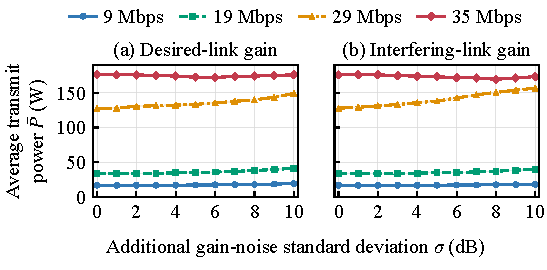
\includegraphics[width=\columnwidth]{figures/gain_error_power_revision1.pdf}
    \caption{\rev{Sensitivity of the average system transmit power $\bar{P}$ to gain-prediction errors.}}
    \label{fig:gain-error-power}
\end{figure}

\rev{This subsection evaluates how gain-prediction errors affect the system transmit power and latency performance of MEET-COBRA. We add independent zero-mean Gaussian noise with standard deviation $\sigma\in\{0,1,\ldots,10\}$~dB to either the original desired-link or interfering-link gain predictions. Keeping the trained models, beam-pair candidates, actual channels and traffic arrivals unchanged, we rerun MEET-COBRA at $\lambda\in\{9,19,29,35\}$~Mbps with three paired random seeds.}

\rev{Fig.~\ref{fig:gain-error-sensitivity} shows that $U$ changes little at $9$ and $19$~Mbps for $\sigma\leq5$~dB. With $\sigma=5$~dB, $U$ at $29$~Mbps increases from $0.19\%$ to $0.29\%$ when noise is added to either type of gain prediction. At $35$~Mbps, however, adding noise with $\sigma=5$~dB raises $U$ from $1.15\%$ to $3.84\%$ and $3.13\%$ for desired-link and interfering-link gain predictions, respectively.}

\rev{Fig.~\ref{fig:gain-error-power} shows that larger gain-prediction errors generally increase transmit power at the three lower traffic loads. At $19$~Mbps, adding noise with $\sigma=10$~dB to the interfering-link gain predictions increases power from $33.80$ to $40.15$~W, while $U$ remains approximately $0.24\%$. At $35$~Mbps, however, power remains close to the full-load level while $U$ rises sharply.}

\rev{We further study the influence of gain-prediction errors on HO and beam probing. At $29$~Mbps, adding noise with $\sigma=5$~dB to the desired-link gain predictions increases the mean number of HOs per frame from $3.70$ to $20.01$ and the mean number of probes per beam search from $1.06$ to $1.95$. These additional HOs and beam probes reduce the time available for data transmission. At high loads, limited remaining RB resources make it harder to compensate for this loss of transmission time through additional RB allocation.}

\section{Conclusion}

This paper proposed MEET-COBRA, a ML-based energy-efficient proactive coordination framework for jointly optimizing PHO, BF and RA in HetNets.
By leveraging ML-based prediction of beam-pair candidates and channel gains, MEET-COBRA provides a low-complexity online approach to efficiently address the two-timescale SINLP for COBRA.

Simulations driven by SUMO mobility traces and Sionna RT channel data validate the effectiveness of MEET-COBRA.
\currentdel{The ML-driven proactive optimization mechanism delivers substantial gains: the}\rev{The} predicted beam-pair and channel gain information enables efficient global PHO optimization, reduces beam-search overhead, and mitigates RB wastage and latency constraint violations caused by suboptimal BF and RA decisions, thereby addressing the computational challenges of the two-timescale SINLP in practical deployments. 
Notably, MEET-COBRA effectively balances system transmit power and \currentdel{latency reliability}\rev{latency performance}\currentdel{: at}\rev{. At} an illustrative medium-to-high load operating point ($\lambda=27$~Mbps), it reduces the average system transmit power by approximately \currentdel{32\%}\rev{49\%} compared with the Reactive-OBRA baseline, while decreasing the latency constraint violation probability from \currentdel{29.47\% to 0.68\%}\rev{9.84\% to 0.16\%}.
\rev{Compared with the baselines adapted from \cite{wang2024joint} and \cite{heydarian2025multitimescale}, MEET-COBRA uses less transmit power at light and medium loads and achieves lower latency constraint violation probabilities at high loads.}
\rev{It also maintains low violation probabilities under moderate additional gain-prediction errors at light and medium loads.}
%It demonstrates that proactive coordination is essential for sustaining high-performance communication in demanding V2X environments.

Potential future work includes extending MEET-COBRA to multi-macro BS deployments, \currentdel{incorporating more realistic HO latency and signaling overhead}\rev{modeling HO failure recovery and detailed signaling procedures}, and developing online adaptation mechanisms for the prediction models and algorithm hyper-parameters to enhance robustness under non-stationary traffic and radio environments.



\bibliographystyle{IEEEtran}
\bibliography{reference.bib}%%我们的例子应该是\bibliography{cited}

\end{document}
